% Options for packages loaded elsewhere
\PassOptionsToPackage{unicode}{hyperref}
\PassOptionsToPackage{hyphens}{url}
%
\documentclass[
]{book}
\usepackage{amsmath,amssymb}
\usepackage{lmodern}
\usepackage{iftex}
\ifPDFTeX
  \usepackage[T1]{fontenc}
  \usepackage[utf8]{inputenc}
  \usepackage{textcomp} % provide euro and other symbols
\else % if luatex or xetex
  \usepackage{unicode-math}
  \defaultfontfeatures{Scale=MatchLowercase}
  \defaultfontfeatures[\rmfamily]{Ligatures=TeX,Scale=1}
\fi
% Use upquote if available, for straight quotes in verbatim environments
\IfFileExists{upquote.sty}{\usepackage{upquote}}{}
\IfFileExists{microtype.sty}{% use microtype if available
  \usepackage[]{microtype}
  \UseMicrotypeSet[protrusion]{basicmath} % disable protrusion for tt fonts
}{}
\makeatletter
\@ifundefined{KOMAClassName}{% if non-KOMA class
  \IfFileExists{parskip.sty}{%
    \usepackage{parskip}
  }{% else
    \setlength{\parindent}{0pt}
    \setlength{\parskip}{6pt plus 2pt minus 1pt}}
}{% if KOMA class
  \KOMAoptions{parskip=half}}
\makeatother
\usepackage{xcolor}
\usepackage{longtable,booktabs,array}
\usepackage{calc} % for calculating minipage widths
% Correct order of tables after \paragraph or \subparagraph
\usepackage{etoolbox}
\makeatletter
\patchcmd\longtable{\par}{\if@noskipsec\mbox{}\fi\par}{}{}
\makeatother
% Allow footnotes in longtable head/foot
\IfFileExists{footnotehyper.sty}{\usepackage{footnotehyper}}{\usepackage{footnote}}
\makesavenoteenv{longtable}
\usepackage{graphicx}
\makeatletter
\def\maxwidth{\ifdim\Gin@nat@width>\linewidth\linewidth\else\Gin@nat@width\fi}
\def\maxheight{\ifdim\Gin@nat@height>\textheight\textheight\else\Gin@nat@height\fi}
\makeatother
% Scale images if necessary, so that they will not overflow the page
% margins by default, and it is still possible to overwrite the defaults
% using explicit options in \includegraphics[width, height, ...]{}
\setkeys{Gin}{width=\maxwidth,height=\maxheight,keepaspectratio}
% Set default figure placement to htbp
\makeatletter
\def\fps@figure{htbp}
\makeatother
\setlength{\emergencystretch}{3em} % prevent overfull lines
\providecommand{\tightlist}{%
  \setlength{\itemsep}{0pt}\setlength{\parskip}{0pt}}
\setcounter{secnumdepth}{5}
\usepackage{booktabs}
\usepackage{amsthm}
\makeatletter
\def\thm@space@setup{%
  \thm@preskip=8pt plus 2pt minus 4pt
  \thm@postskip=\thm@preskip
}
\makeatother
\ifLuaTeX
  \usepackage{selnolig}  % disable illegal ligatures
\fi
\usepackage[]{natbib}
\bibliographystyle{apalike}
\IfFileExists{bookmark.sty}{\usepackage{bookmark}}{\usepackage{hyperref}}
\IfFileExists{xurl.sty}{\usepackage{xurl}}{} % add URL line breaks if available
\urlstyle{same} % disable monospaced font for URLs
\hypersetup{
  pdftitle={Cooking After Retirement},
  pdfauthor={Bruce Cochrane},
  hidelinks,
  pdfcreator={LaTeX via pandoc}}

\title{Cooking After Retirement}
\author{Bruce Cochrane}
\date{2022-08-04}

\begin{document}
\maketitle

{
\setcounter{tocdepth}{1}
\tableofcontents
}
\hypertarget{dedication}{%
\chapter*{Dedication}\label{dedication}}
\addcontentsline{toc}{chapter}{Dedication}

My adventures in the kitchen date back to my childhood, and I am actually thankful that neither my mother nor my father (Vince and Jean Cochrane) liked to cook, so they eagerly encouraged my childhood desire to explore. As an adult, my family - both my first wife, the late Barbara Leyden, and my second, Alice Kahn, provided encouragement and constructive criticism where necessary. Finally, my two sons, Steven and John Cochrane, are continuing the cooking tradition - Steven as a vegetarian and John as a budding pitmaster. This book is lovingly dedicated to all of them.

\hypertarget{introduction}{%
\chapter{Introduction}\label{introduction}}

Cooking has always been a big part of my life, but since I retired from my career as a geneticist, I have had more time to explore new areas. In particular, two factors have become central to my culinary efforts:

\hypertarget{bread}{%
\section{Bread}\label{bread}}

I have long been fascinated by sourdough cooking - I successfully made my first starter (on the first try!) in 1974 and managed to keep it going for a few years before moves and inattention doomed it to oblivion. When I moved to Ohio in 2007, my interest was rekindled, especially after I discovered Reinhardt's \emph{Artisanal Bread at Home}. His starter recipe took a couple of trys, but the use of ``organic'' flour and pineapple juice in the initial mix proved successful. That starter is now about 13 years old and going strong (I'll talk about maintenance in the \protect\hyperlink{bread}{Bread} section).

The second piece in by bread baking evolution was a result of my wife's Christmas gift of \emph{Tartines} in 2021. This is a fascinating book, one which interweaves recipes with detailed explanations of the reason for each step and photographs of how the steps are performed. The recipes are fairly involved, and following them from the book involves a lot of page turning (NOT something I'd want to do with an ebook), but the results can be spectacular. Again, I will provide some \protect\hyperlink{tartines}{simplified ideas} to facilitate your efforts.

\hypertarget{the-big-green-egg}{%
\section{The Big Green Egg}\label{the-big-green-egg}}

In 2011, Alice and I embarked on a major project to finish the basement of her (now our) home. So what does this have to do with cooking? Nothing directly, however while shopping for a gas fireplace, we saw our first \href{http://www.biggreenegg.com}{Big Green Egg} and decided we wanted one (she mostly for its appearance, me for the intriguing cooking possibilities). Shortly thereafter, we purchased a medium one, and while we had a lot of fun with it (initially for pizza and baked potatoes), it soon became apparent that we needed a larger one. Accordingly, a few years later, I sprung for a large one. I will have more to say about it in the \protect\hyperlink{bge}{Big Green Egg} section.

Over the subsequent years, my Green Egg recipe portfolio has diversified. Most of what I do can be divided into two categories - grilling and barbecuing. Grilling is what most casual outdoor cooking enthusiasts are most familiar with - cooking over high heat, often with some sort of basting sauce, with cooking times usually measured in minutes. Barbecuing, by contrast, involves ``low and slow'' cooking (temperatures maintained at 150-250\textsuperscript{o} F.) and cook times measured in hours. The results, with properly monitored cooking, can be outstanding.

\hypertarget{other-stuff}{%
\section{Other Stuff}\label{other-stuff}}

But you might say things like ``man doesn't live by bread alone'' or ``what about the winter months?''. Both are valid critiques, so in a subsequent section, I will describe some indoor cooking recipes I've come to depend on. And I'll be quite honest - I really don't go for admittedly healthy options like, perhaps, green bean and kale salad. So I've entitled the chapter \protect\hyperlink{comfort}{Comfort Food}, reflecting the fact that, while the recipes are perhaps not the stuff of a dietician's dream, they are (at least to me) fun to eat. Furthermore, most of them don't require a whole lot of cooking time. Some of them are modifications of ones originally found in cookbooks (which are cited), but which I have modified for either flavor or ease of cooking reasons. A good example of this is the recipe for macaroni and cheese - the sauce is originally from the venerable \emph{Joy of Cooking} but modified to increase the spiciness and make use of a microwave oven.

\hypertarget{a-note-on-portion-size-and-original-sources}{%
\section{A Note on Portion Size and Original Sources}\label{a-note-on-portion-size-and-original-sources}}

Everyone is familiar with estimated serving numbers in published recipes. In general, I find them to be rather inaccurate, so when trying a new recipe, I use them at most for a rough guideline. And personally, what I found to be a single serving for me 50 years ago is a serving plus leftovers or even two servings for me today. All of the recipes I've included are of that size; you of course may find otherwise.

And finally, I will confess that there are almost no purely original recipes in this book - all are ones that were originally obtained from either a cookbook or an online source. Those sources are cited in the recipes themselves, and all sources, with brief annotations, are provided in the {[}concluding chapter{]}.

\hypertarget{essentials}{%
\chapter{Kitchen Essentials}\label{essentials}}

So the bad news is that there is an enormous number of kitchen gadgets, utensils, dishes, bowls and table top appliances out there eager to drain your wallet. The good news? You don't need most of them. Beyond the items found in every kitchen (stove, refrigerator, mixing bowls, etc.) there are only a few items that will make your life easier, and in fact you can cook perfectly adequately without them. Here are a few that I use on a regular basis.

\hypertarget{bread-making}{%
\section{Bread Making}\label{bread-making}}

The following can be done without, but I consider them to be all but essential.

\begin{enumerate}
\def\labelenumi{\arabic{enumi}.}
\tightlist
\item
  \textbf{A stand mixer}. The two cookbooks I recommend in the \protect\hyperlink{bread}{Bread} section have different takes on this. Reinhardt calls for using one in almost every recipe, while I'm pretty sure that Robertson (\emph{Tartines}) doesn't even mention them. I happen to use one wherever possible, even when the recipe doesn't call for it (and will do do so throughout the recipes). Ours is a Viking that, as far as I can tell, is no longer being manufactured (although you may find a used one available on ebay or some similar site). The much more common ones, of course, are those of \href{https://www.kitchenaid.com/countertop-appliances/stand-mixers.html}{Kitchenaid}, definitely fine machines. They come in two sizes , 4 qt. and 5.5 qt. I received one of the former as a wedding present 40 years ago, and it served all of my needs at the time just fine (indeed, it is now at my lakefront cottage in the Finger Lakes and still going strong. Were I to buy one today (or if our Viking dies), I would probably go with the larger one.
\item
  \textbf{A kitchen scale}. Most breadmakers will recommend that weight be used to measure ingredients. This is particularly important for flour, since even different bags of the same brand can have different densities. You can get a decent electronic one for around \$25.
\end{enumerate}

\hypertarget{grilling}{%
\section{Grilling}\label{grilling}}

Of course, you will need the \textbf{basic grilling tools} - spatula, fork, tongs and heavy oven mitts. And a cleaning brush. Beyond those I would recommend a \textbf{grilling basket} and a \textbf{fish grilling mesh}. In both cases, be sure you get ones with removable handles, since they won't fit inside a closed Green Egg with the handles on. An example of a grilling basket is \href{https://www.williams-sonoma.com/products/outset-chefs-outdoor-grill-basket-skillet-handles/}{this one from Williams Sonoma}.

\hypertarget{indoor-cooking}{%
\section{Indoor Cooking}\label{indoor-cooking}}

In general, all you need here is a decent selection of pots, pans and bowls. However, I do recommend considering the following:

\begin{enumerate}
\def\labelenumi{\arabic{enumi}.}
\tightlist
\item
  An \textbf{immersion blender}. I never really thought about one of these until I heard an NPR piece on possible Christmas gifts for the cooks in one's life. I immediately thought of my younger son John, so I got him one and he liked it. I subsequently purchased one for myself, a Braun, that is not only a blender but can also be a small blender and chopper, useful for things like grating hard cheese and chopping garlic.
\item
  A \textbf{slow cooker}. This is definitely a secondary priority, since most recipes that call for one can easily be adapted for the stove top or oven. However, it is nice to be able to throw a meal together and forget about it for a few hours. I've included some recipes that use it, but I've also made suggestions as to how to cook them conventionally.
\item
  A \textbf{convection toaster oven} In the summer months, it's nice to be able to cook in one of these and avoid heating up the house by using the oven.\\
\item
  Only a few of these recipes call for using a \textbf{microwave oven}, but one is great to have, especially for thawing and warming leftovers.\\
\item
  Finally, you may ask, what about an \textbf{Instant Pot} or the equivalent. A couple of comments: First, these are at their core programmable pressure cookers. I've used stove top pressure cookers on and off for years, so I understand their allure. However, while I do have one in my lake house in New York, I've never gotten around to buying one for our Ohio home. I've included one recipe (for \protect\hyperlink{fajitas}{fajitas} that I particularly like, but it can also be prepared on the grill. So if you want to, go for it - the internet has almost as many IP recipes as it does cat videos, so there will be a lot for you to explore.
\end{enumerate}

\hypertarget{bread-1}{%
\chapter{Bread}\label{bread-1}}

\hypertarget{getting-started}{%
\section{Getting Started}\label{getting-started}}

While I've tried to include everything you need to know in order to bake all of these recipes, I have not included a lot of background information on the whys and wherefores of the processes. For that, I strongly recommend that you purchase the following two books And get physical books, not ebooks. Ebooks are not good for all the page-flipping you will want to do.

\begin{enumerate}
\def\labelenumi{\arabic{enumi}.}
\tightlist
\item
  \emph{Artesan Bread at Home} by Peter Reinhardt. This is the book I started with, and it remains a go-to source. It walks you through \protect\hyperlink{starter}{making and maintaining starter}, and my recipes for \protect\hyperlink{pal}{Pan au Levain} and \protect\hyperlink{pizzadough}{pizza dough} originated there. There are lots of other good recipes (both sourdough and conventional) that you may want to try.
\item
  \emph{Tartines}, by Chad Robertson. This book took me to the next step of sourdough baking. It is a different kind of book, in that a) it is very autobiographical, an b) it is mostly built around \protect\hyperlink{tartines}{a single recipe}. It is also extremely well illustrated, so I'd suggest having it at hand when you follow my condensed versions of his recipes.
\end{enumerate}

\hypertarget{what-you-will-need}{%
\section{What you will need}\label{what-you-will-need}}

\hypertarget{flour}{%
\subsection{Flours}\label{flour}}

Volumes gave been written on the virtues and shortcoming of all kinds of flour. For the casual baker, but of that can be ignored, however there are a few basics that need to be kept in mind.

\hypertarget{sources}{%
\subsubsection{Sources}\label{sources}}

I have the good fortune of having access to an excellent bulk food store (Sauder's Store in Seneca Falls, NY), so I can buy 25 pound bags of flour for about \$18.00. Because I can only get there a couple of times a year, I usually buy 2-3 bags and them store them in a sealed plastic tub. I've never had any problems with weevils. If you live near a similar source, go for it. However, if you don't, King Arthur varieties are always good (for high gluten choices, ``Bread Flour'' works well; their ``Sir Lancelot'' is the best).

\hypertarget{bread-vs.-all-purpose.}{%
\subsubsection{Bread vs.~All Purpose.}\label{bread-vs.-all-purpose.}}

The big difference here is gluten. Fortunately, none of my family have any problems with gluten, so my motto is the more the merrier. This is where bread flour comes in - it is simply white flour that is high in gluten. Use of bread flour leads to a more elastic dough and a more open texture of the resulting loaf.

\hypertarget{whole-wheat-flour}{%
\subsubsection{Whole Wheat Flour}\label{whole-wheat-flour}}

I've never been a fan of 100\% whole wheat bread, however adding a small amount (maybe 10-20\% of the total) tends to improve the flavor (and perhaps marginally the nutritional value) of most bread recipes. It is an essential part of both Pan au Levain and Essential Tartine Bread, and can be added to most of the other recipes (however I don't recommend it for Dinner Rolls, and adding it to pizza dough is a matter of taste). It pays to get high quality stone ground whole wheat flour - you'll pay a little more for it, but one bag goes a long way.

\hypertarget{starter}{%
\section{Making the starter}\label{starter}}

\hypertarget{getting-it-started}{%
\subsection{Getting it Started}\label{getting-it-started}}

\hypertarget{maintaining-and-recharging}{%
\subsection{Maintaining and Recharging}\label{maintaining-and-recharging}}

Reinhardt recommends recharging the mother starter at least once a week. I find that not to be necessary (at least with my starter) - doing so every 3-4 weeks has proven to be adequate. However, my qualitative observation is that the longer I've left it in the refrigerator, the longer the recharge fermentation takes. Only once or twice has following the recipe below failed; in that case I go back to step xxx in the process I used to make the starter in the first place and go from there. The normal recharge procedure is as follows:

\begin{quote}
2 3/4 cups bread flour (add some whole wheat if you like)\\
1 cup warm water\\
3/4 cup mother starter
\end{quote}

\begin{enumerate}
\def\labelenumi{\arabic{enumi}.}
\tightlist
\item
  Mix all of the ingredients together using a non-metalic spoon/spatula or your fingers.\\
\item
  Transfer to a clean ceramic bowl and cover with food service wrap
\item
  Place in a warm place overnight, or until the starter has nearly doubled in bulk and is very bubbly.
\item
  Transfer to a sealed food storage container and store in the refrigerator. I do recommend labeling the container with the date it was made.
\end{enumerate}

\hypertarget{recipes}{%
\section{Recipes}\label{recipes}}

\hypertarget{pal}{%
\subsection{Pan au Levain}\label{pal}}

This is our go-to Reinhardt-style bread, and I give him all of the credit for suggesting the ingenious trick of adding whole wheat flour to the starter. My addition was to hybridize it with the Robertson approach to proofing, shaping and baking. I think you will be more than pleased with the results.

\hypertarget{pizzadough}{%
\subsection{Pizza Dough}\label{pizzadough}}

\hypertarget{rolls}{%
\subsection{Sourdough Rolls}\label{rolls}}

Below are two recipes from Amy Duska at \href{https://littlespoonfarm.com/}{Little Spoon Farms}, a great source for sourdough ideas. Like me, she is self-taught in the art of sourdough baking, and her recipes are geared towards others with similar aspirations. Below are two of her recipes, each with a few tweaks I've incporated.

\hypertarget{drolls}{%
\subsubsection{Dinner Rolls}\label{drolls}}

I cooked these for Thanksgiving dinner, and I anticipate doing so from here on out (as well as any other occasion that calls for them). They are like store-bought dinner rolls, however the sourdough imparts more flavor. Like most of the recipes I've used, this is a three day process - make the starter (overnight), mix the dough and do primary fermentation (day 2), do refrigerated secondary fermantation over night, and shape and bake (day 3).

\hypertarget{day-1}{%
\subsubsection{Day 1}\label{day-1}}

Make the starter as follows:

\begin{quote}
1 tbsp mother starter\\
\textasciitilde1/3 cup flour (either bread or all purpose)\\
3.5 tbsp water
\end{quote}

Combine the above in a small bowl, cover with food service wrap, and let it rise in a warm place overnight.

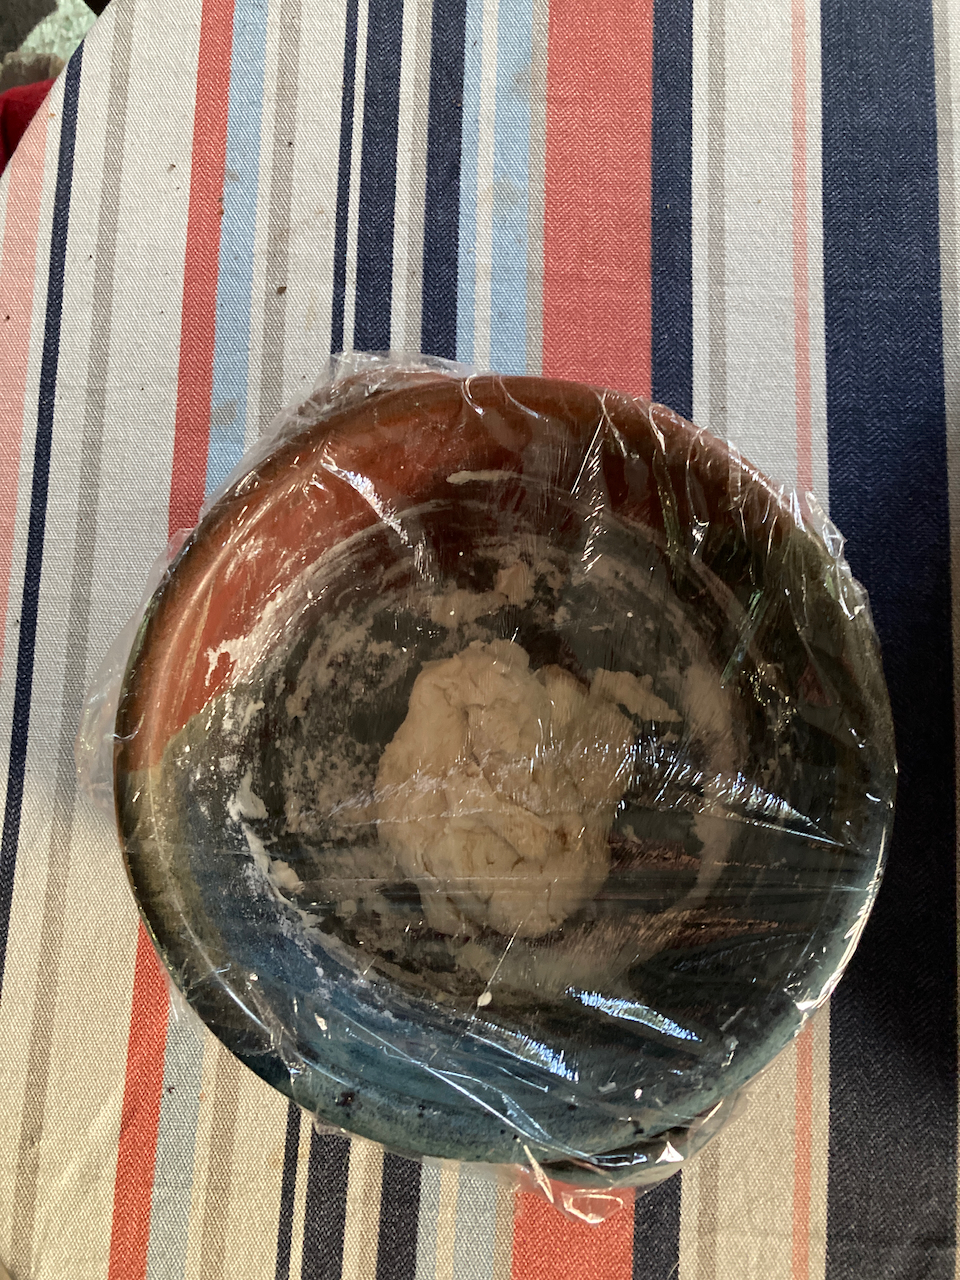
\includegraphics[width=0.4\textwidth,height=\textheight]{images/rollstarter1.jpeg}
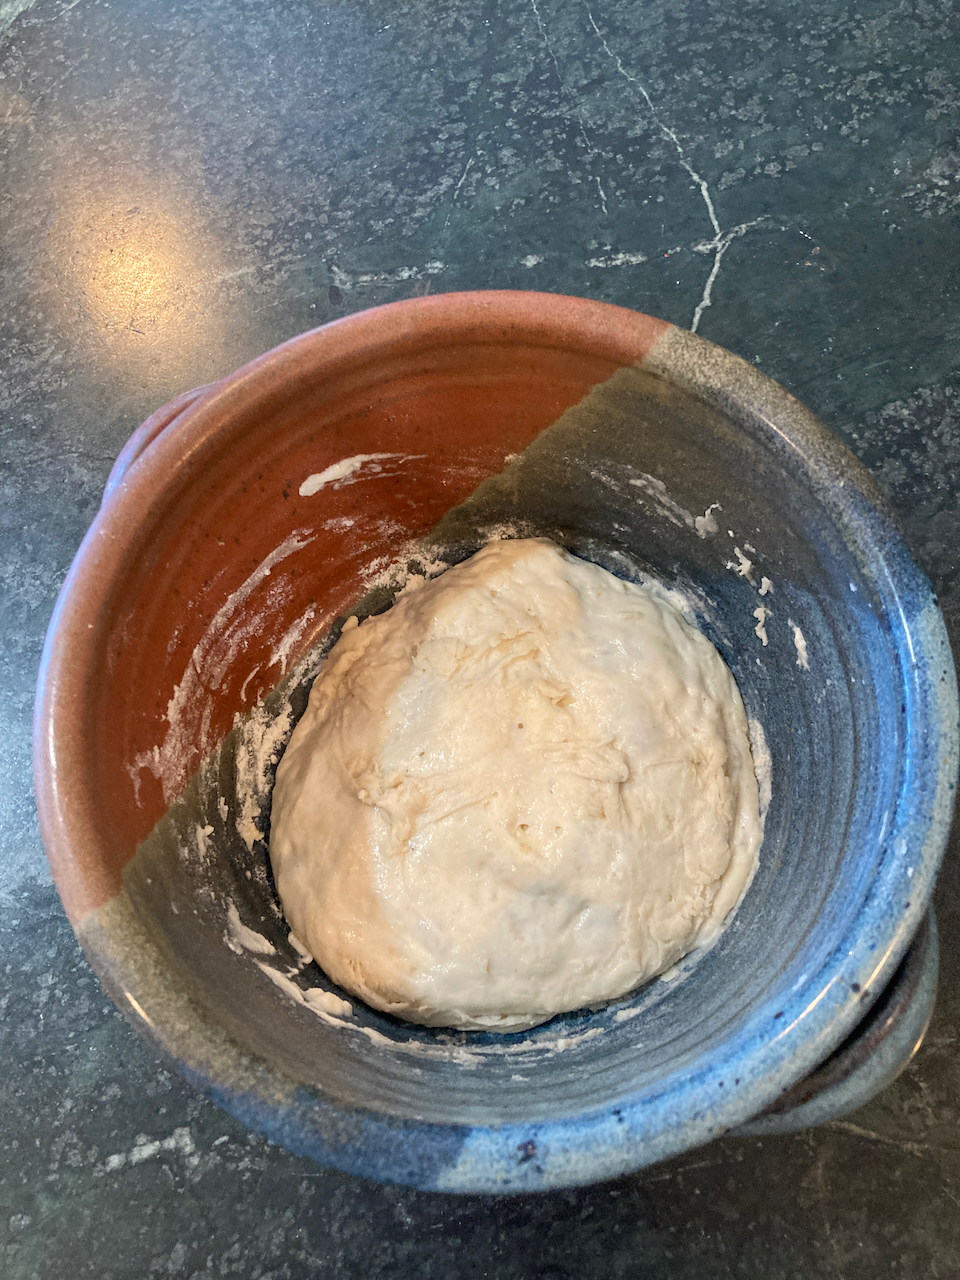
\includegraphics[width=0.4\textwidth,height=\textheight]{images/rollstarter2.jpeg}

Starter Before and After Overnight Fermentation

\hypertarget{day-2}{%
\subsubsection{Day 2}\label{day-2}}

Dough ingredients:

\begin{quote}
2 tbsp melted butter\\
1 cup (240 gm) milk\\
3 tbsp (44 gm) sugar\\
1 tsp (5 gm) salt\\
1/2 cup (100 gm) starter\\
3 cups + 2 tbsp (375 gm) bread flour\\
1 tbsp melted butter to brush on surface after baking
\end{quote}

Mixing the dough:

\begin{enumerate}
\def\labelenumi{\arabic{enumi}.}
\tightlist
\item
  Combine butter, sugar, milk and salt and warm over low heat until butter is melted. transfer to mixer bowl and let cool to room temperature.
\item
  Add flour and starter and mix with paddle attachment at low speed, until the ingredients are mixed and hydrated.
\item
  Transfer dough to a ceramic bowl, cover with a dish towel, and let it stand for an hour.
\item
  Now comes our first exposure to tartine-style stretching and folding. Uncover the dough, and with moistened clean hands, pick up the dough from one side, stretch it a bit, and fold over what's in the bowl. Repeat this process three times, rotating the bowl 1/4 turn before each one.
\item
  Repeat step four two more times, allowing 30 minutes of rising time between each stretch and fold.
\item
  Cover the bowl with food service wrap and refrigerate overnight.
\end{enumerate}

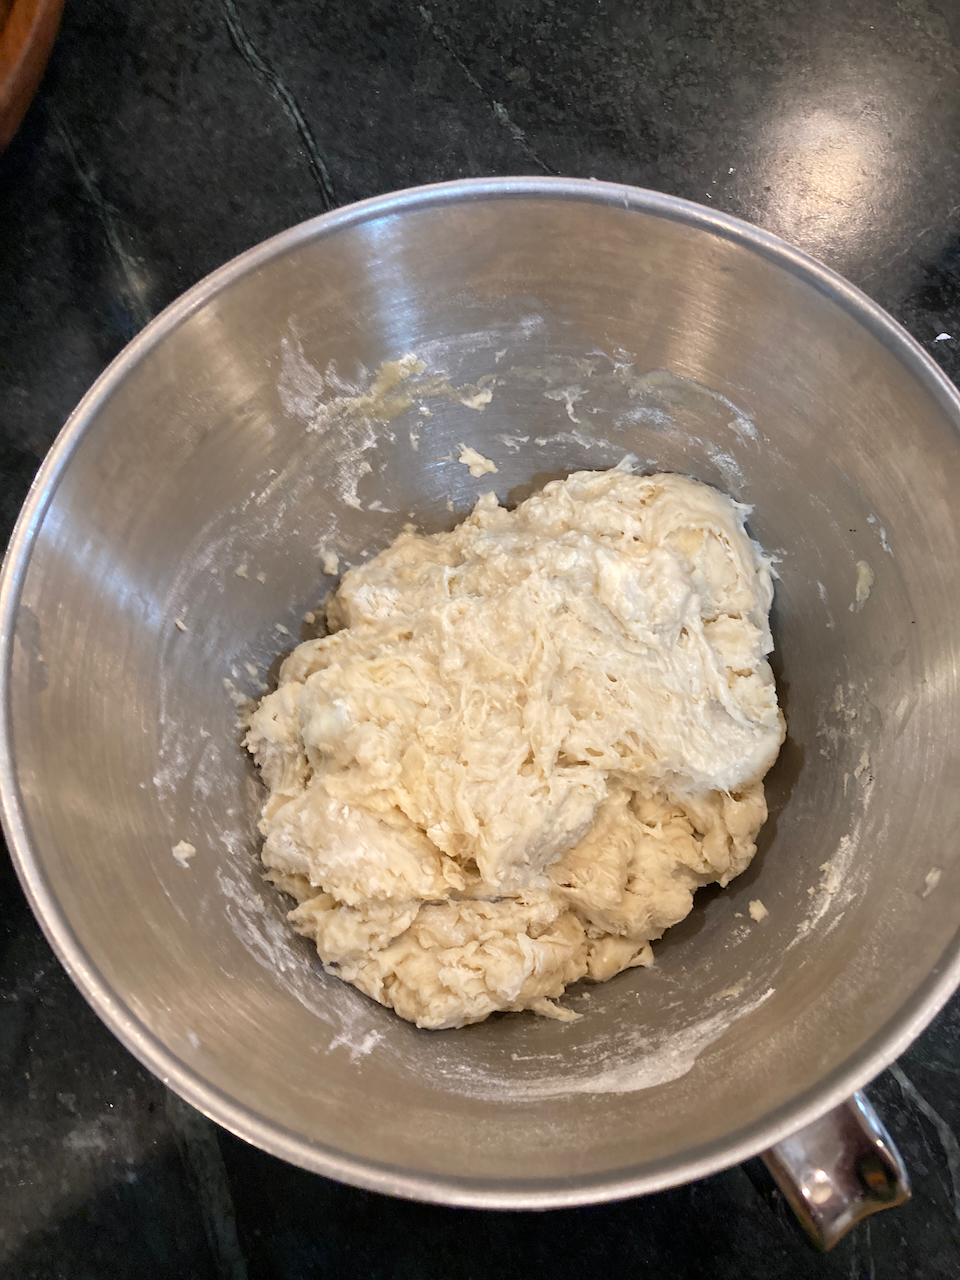
\includegraphics[width=0.7\textwidth,height=\textheight]{images/drolls1.jpeg}

After initial mixing

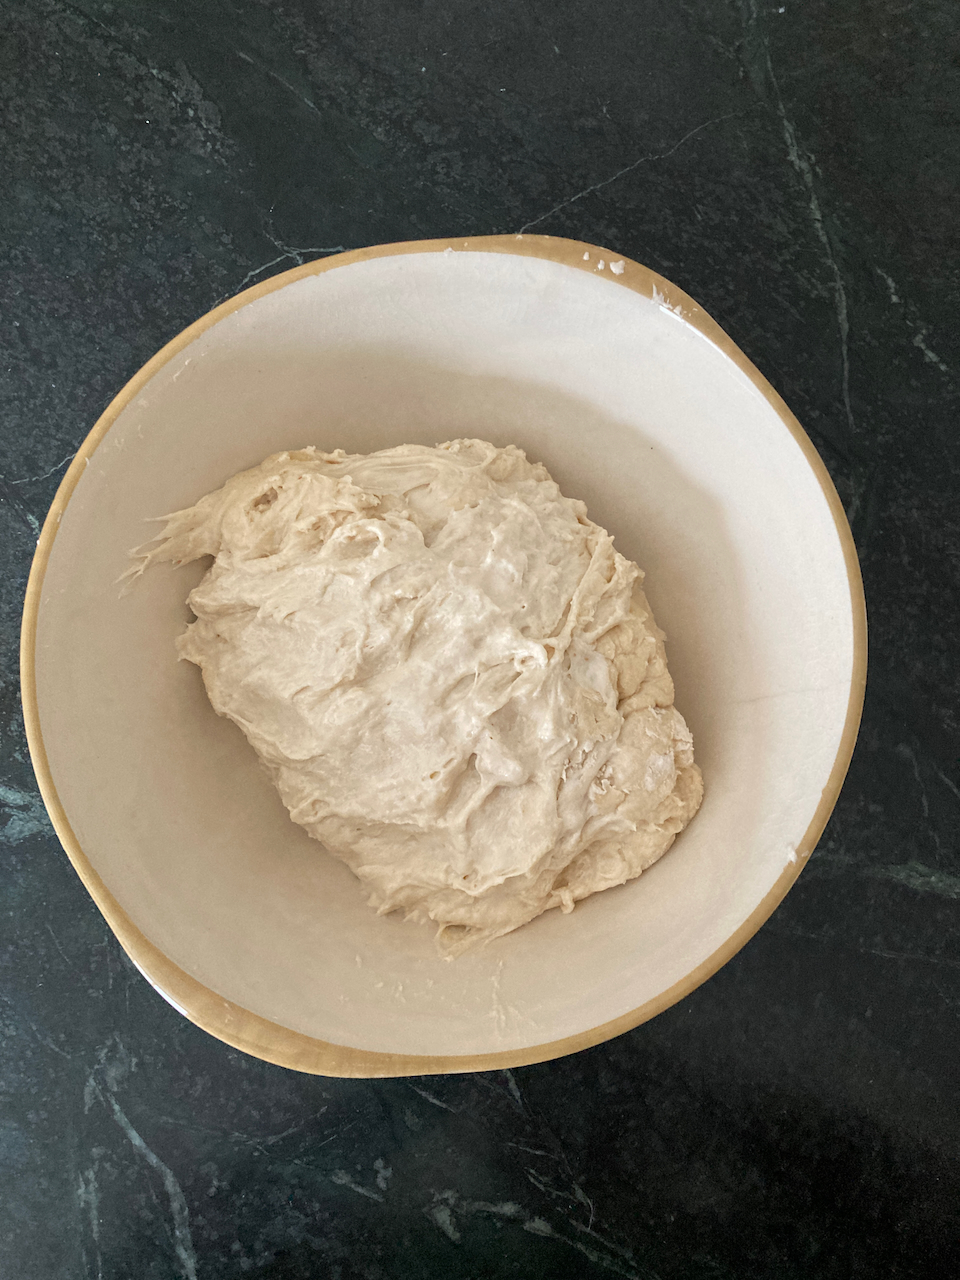
\includegraphics[width=0.4\textwidth,height=\textheight]{images/drolls2.jpeg}
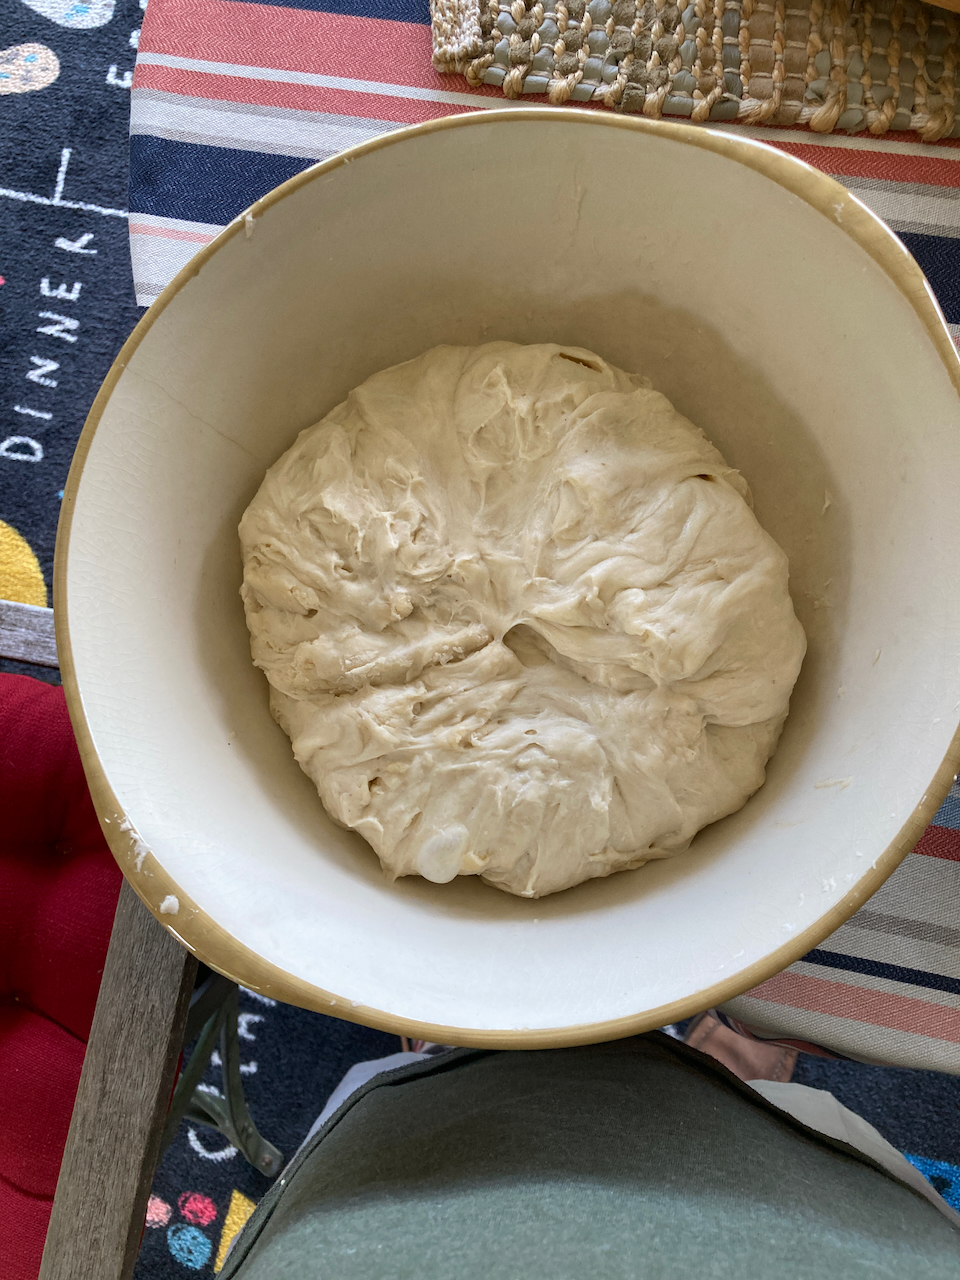
\includegraphics[width=0.4\textwidth,height=\textheight]{images/drolls3.jpeg}

Dough before (left) and after (right) stretching and folding. Note that the dough has expanded in volume and has a smoother surface. It also becomes much more elastic.

\hypertarget{day-3}{%
\subsubsection{Day 3}\label{day-3}}

Today is shaping and baking day, a good day to plan for delicious fresh rolls with dinner!

\begin{enumerate}
\def\labelenumi{\arabic{enumi}.}
\tightlist
\item
  Remove the dough from the refrigerator and let it warm 1-2 hours.
\item
  Put dough on a surface dusted with rice flour and divide into 12 roughly equal pieces of \textasciitilde65 grams each.
\item
  Shape each piece into a ball by turning up the sides and pinching them together. Arrange in a 9 X 13 inch baking dish dusted with rice flour (either a glass or a ceramic dush will work), cover with a towel, and let rise 3-4 hours.
\item
  Preheat your oven to 375\textsuperscript{o} F. Brush the surface of the rolls with melted butter and bake 25-30 minutes until golden brown.
\end{enumerate}

\hypertarget{parmesan-bubble-loaf}{%
\subsection{Parmesan Bubble Loaf}\label{parmesan-bubble-loaf}}

This is a combination of three recipes, the \protect\hyperlink{drolls}{dinner roll} recipe we've already seen, the recipe from another old but excellent cookbook - \emph{A World of Breads} by Dolores Casella, and the technique for making cheese breads from Reinhart. We used the first to make the dough and the others to process and bake the dough.

Note that this recipe, as given previously, makes enough dough for one loaf. I usually double everything to make two - one to eat right away (it doesn't last long!) and one to freeze for later.

\emph{Ingredients}

\begin{quote}
A batch of \href{$drolls}{dinner roll dough}, processed through Day 2 (in other words, substitute the following for the Day 3 instructions).\\
1/2 cup parmesan cheese, grated. (3/4 cup if doubled)\\
2 cloves garlic, grated or smashed (3 if doubled)\\
1/2 cup butter (3/4 if doubled)
1 batch dough
\end{quote}

\begin{enumerate}
\def\labelenumi{\arabic{enumi}.}
\tightlist
\item
  After the dough has warmed from its overnight fermentation, gently flatten it on a floured work surface
\item
  Fold in the parmesan, divide the dough into 14 pieces and shape into balls.

  \begin{itemize}
  \tightlist
  \item
    \emph{If you are doing a double batch, divide it into two halves and process each as above.}
  \end{itemize}
\item
  Melt the butter, add the garlic and cook briefly.
\item
  Lightly oil a standard bread loaf pan. Roll each ball of dough in the garlic/butter mix and stack in the loaf pan.
\item
  Cover with a kitchen towel and allow it to rise 3-4 hours.
\item
  Bake at 400\textsuperscript{o} F. for \textasciitilde45 minutes until the top of the loaf is golden brown.
\end{enumerate}

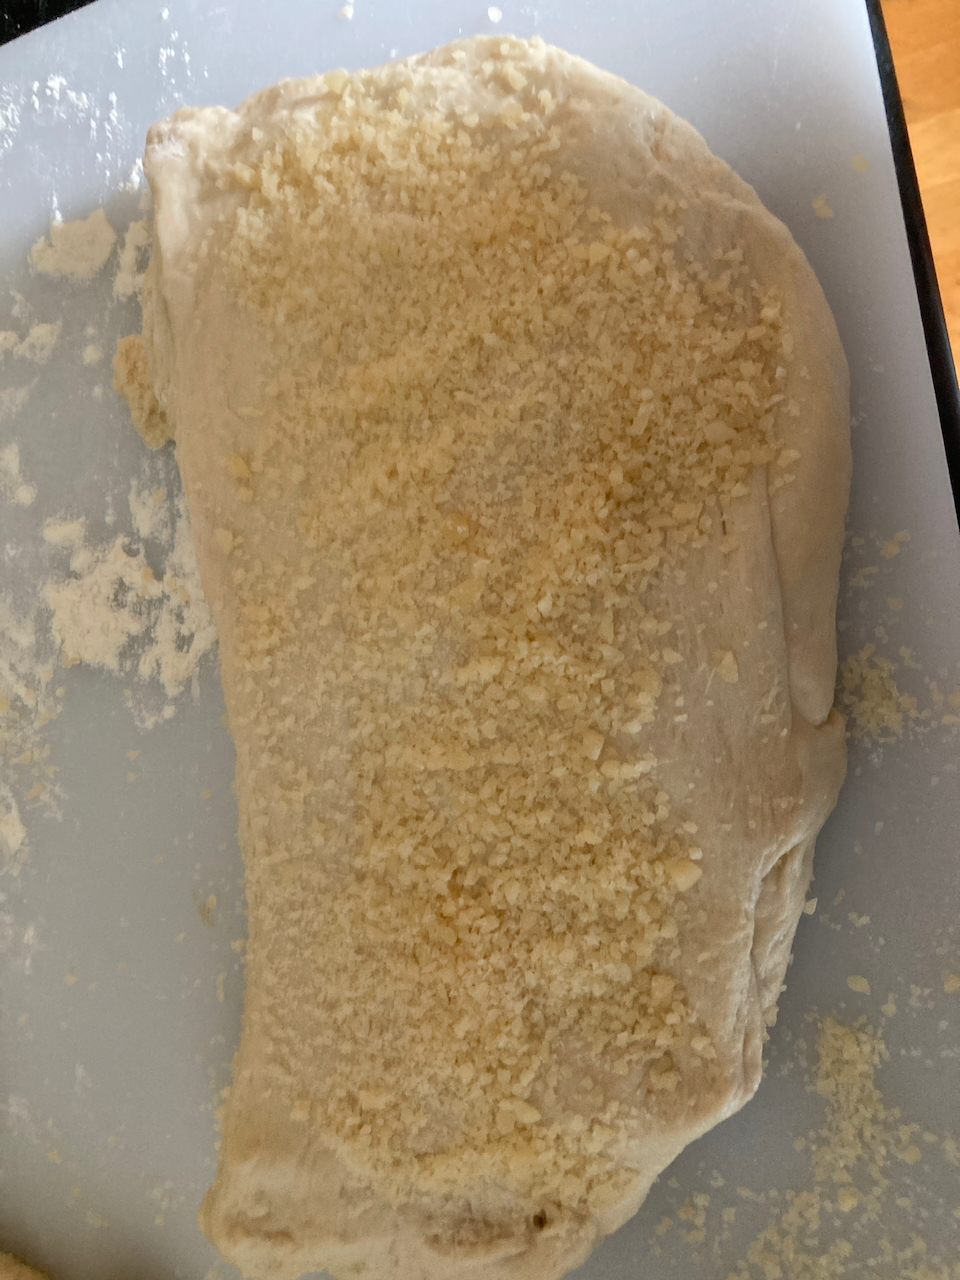
\includegraphics[width=0.7\textwidth,height=\textheight]{images/drolls4.jpeg}

Flattened dough with cheese sprinkled on it.

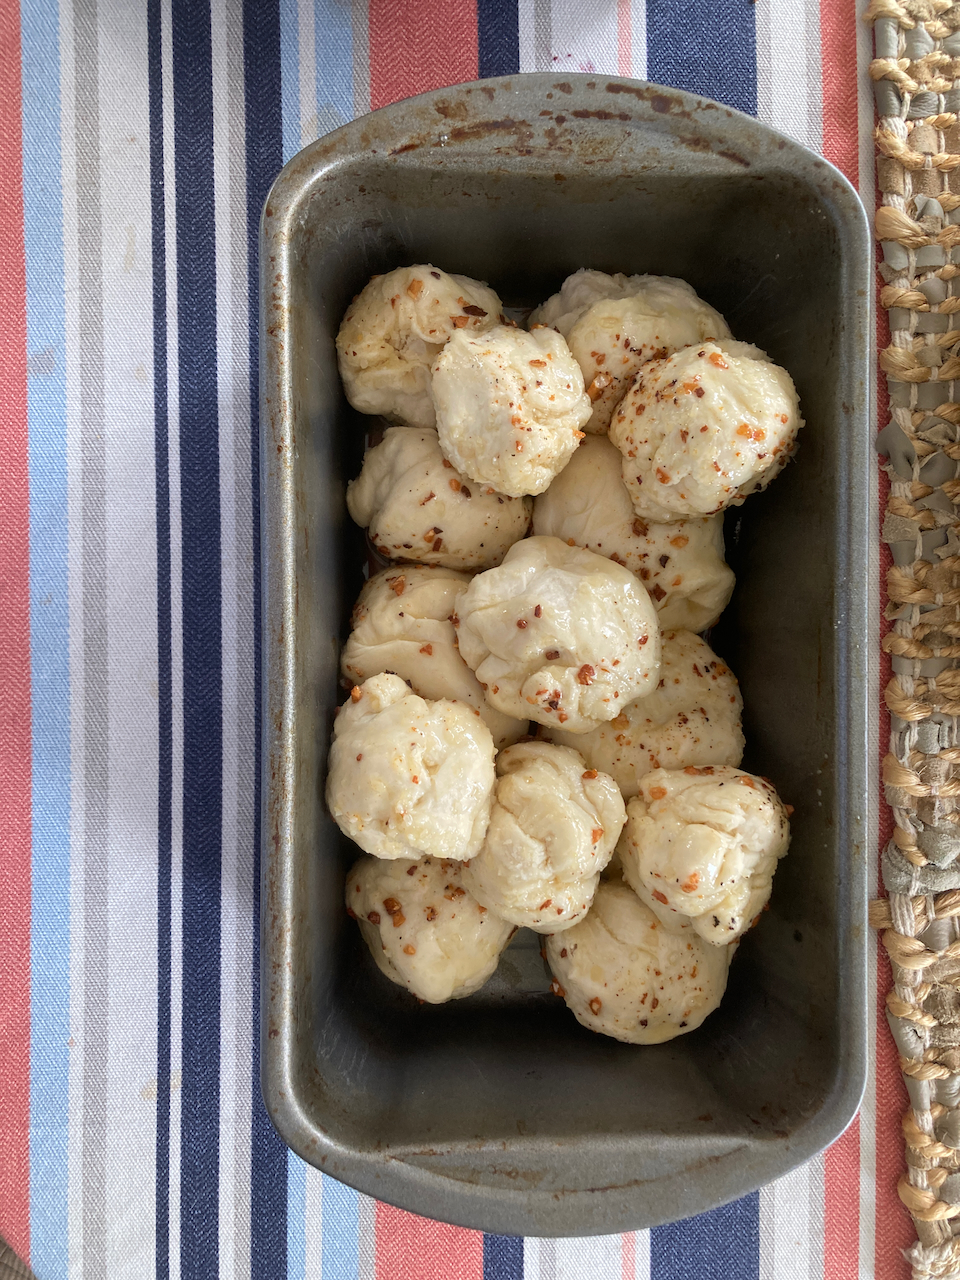
\includegraphics[width=0.35\textwidth,height=\textheight]{images/drolls5.jpeg} 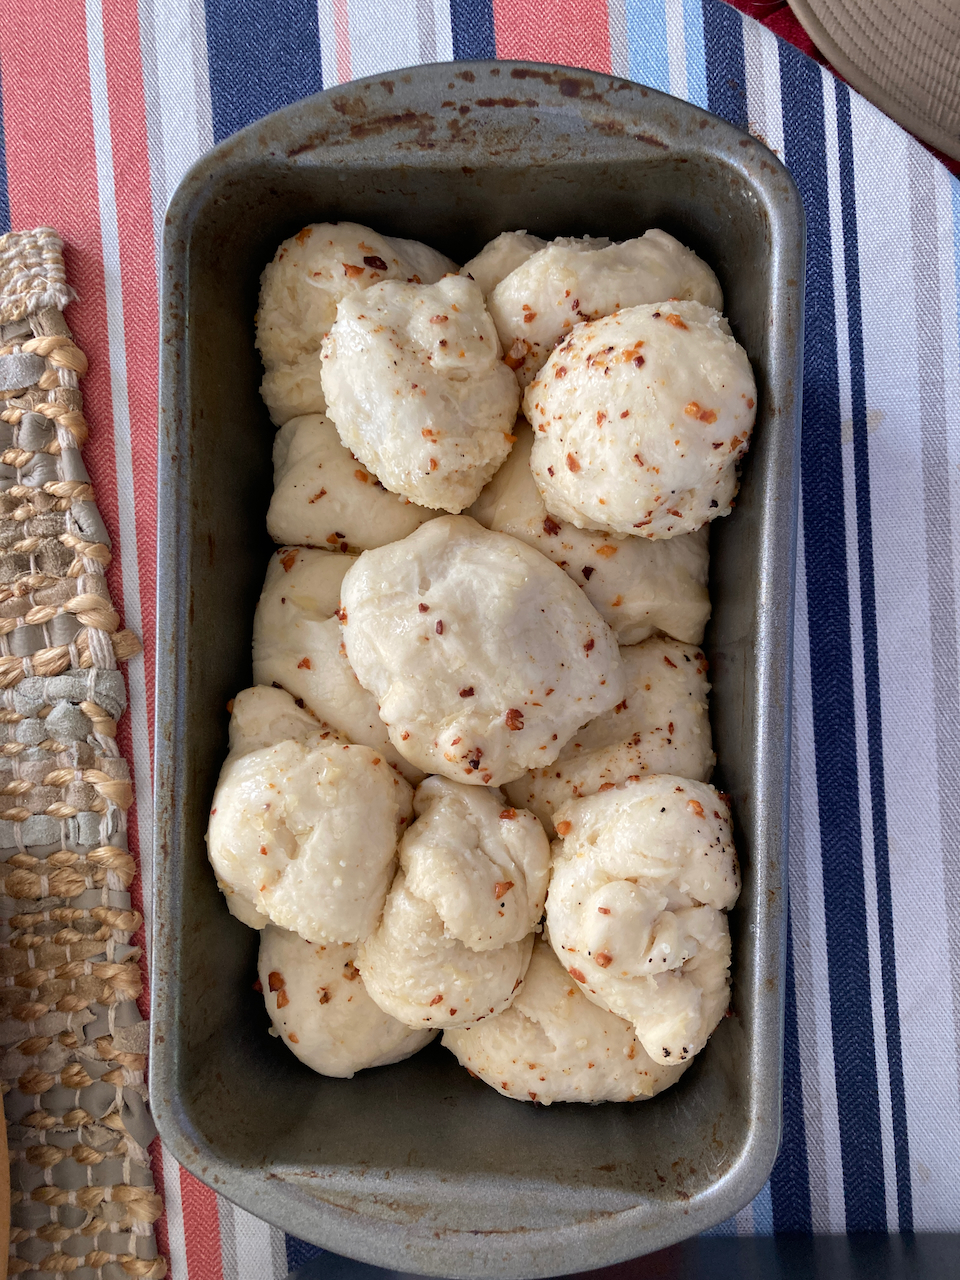
\includegraphics[width=0.35\textwidth,height=\textheight]{images/drolls6.jpeg}

Unbaked loaf before and after the final rise.

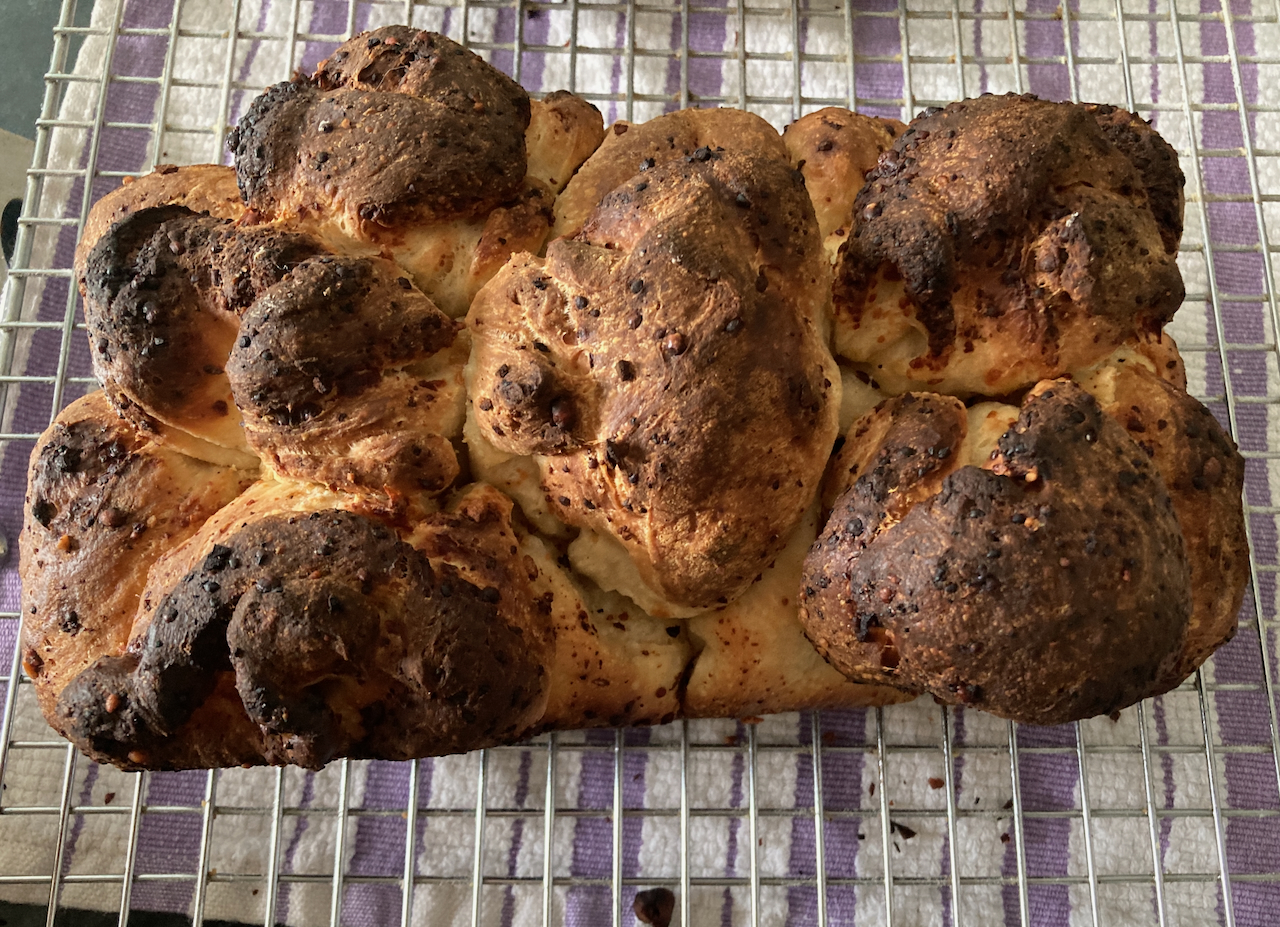
\includegraphics[width=0.8\textwidth,height=\textheight]{images/drolls7.jpeg}

The final product

\hypertarget{ciabatta-rolls}{%
\subsection{Ciabatta rolls}\label{ciabatta-rolls}}

\hypertarget{tartines}{%
\subsection{Essential Tartine Bread}\label{tartines}}

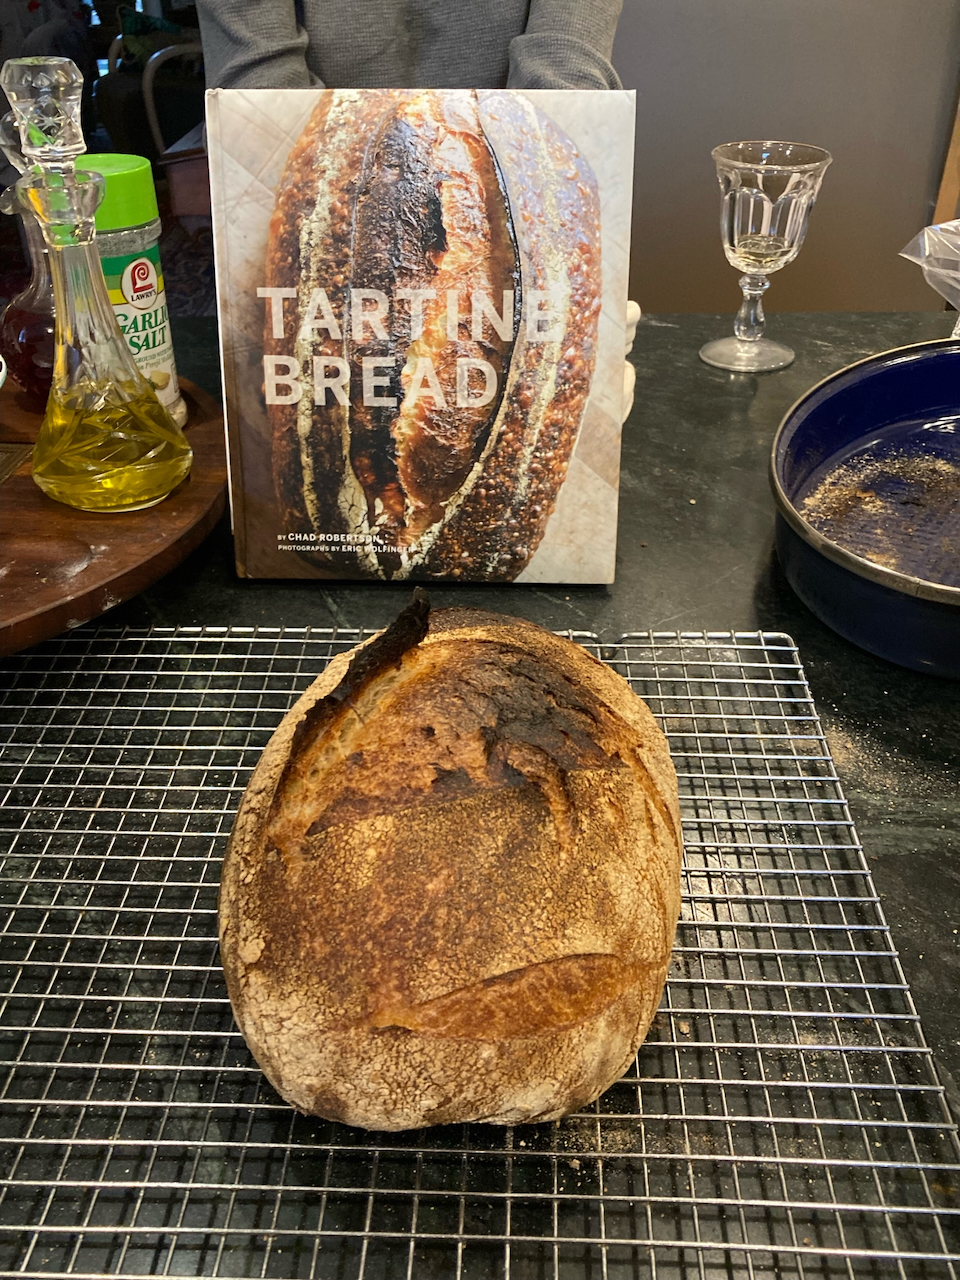
\includegraphics[width=0.5\textwidth,height=\textheight]{images/FirstTartine.jpeg}

My first loaf and the source of the
recipe

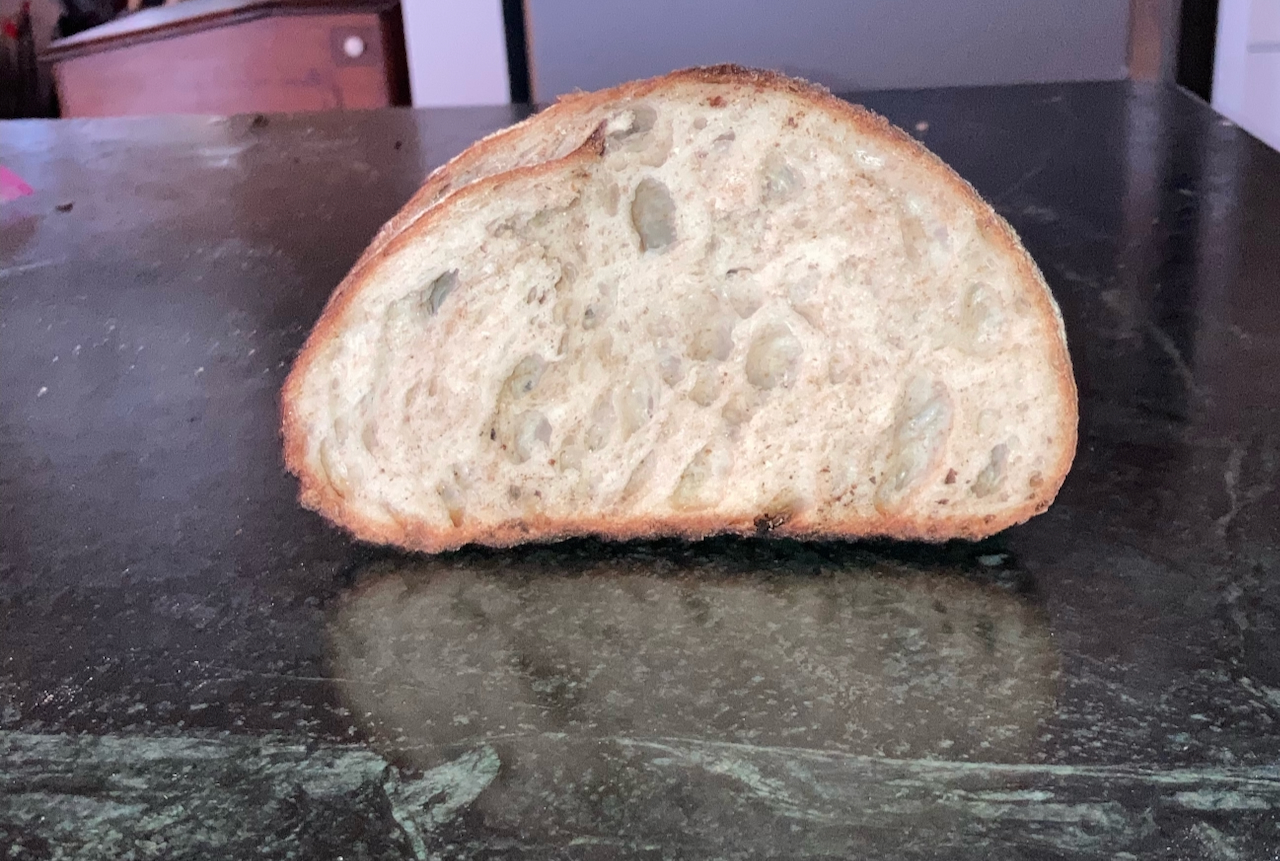
\includegraphics[width=0.7\textwidth,height=\textheight]{images/Tartine2.jpeg}

On the inside, showing the open crumb that results from careful handling of the dough.

\hypertarget{baguettes}{%
\subsection{Tartine Baguettes}\label{baguettes}}

\hypertarget{bge}{%
\chapter{Big Green Egg}\label{bge}}

So what is a Big Green Egg? A more generic name is a komodo cooker - a heavy duty ceramic charcoal cooker, shaped like the ubiquitous Weber Cooker, but much heavier and more expensive. If your budget can afford it, I recommend spending the bucks for an Egg, especially if you anticipate doing a lot of low temperature barbecuing. It is much easier to control the temperature than in a Weber-style device, and a load of charcoal goes a lot longer (an 18 hour barbecue of pork butt or brisket can be completed on a single generous charcoal load). Also, with proper handling, one will last forever, so that while the upfront costs are a challenge, over time you may end up saving money - in my prior life, I found that metal cookers had a lifespan of something like 3-5 years.

With respect to what size to get, I strongly recommend the large (original) Egg. As I mentioned earlier, we started with a medium (recommended for cooking for 2) but quickly found it to be overly constraining - I could barely fir four ears of \protect\hyperlink{corn}{corn on the cob} into it. Furthermore, you can forget grilling multiple different items at the same time.

\begin{quote}
Note that there is an extra large model, which is huge. If you have a big family or are a grilling fanatic, you might want to consider it, but is is far larger than anything I can foresee ever needing.
\end{quote}

\hypertarget{charcoal-and-lighting}{%
\section{Charcoal and Lighting}\label{charcoal-and-lighting}}

There are two cardinal rules regarding what to use in a Green Egg:

\begin{enumerate}
\def\labelenumi{\arabic{enumi}.}
\tightlist
\item
  \textbf{NEVER use lighter fluid. It will soak into the ceramic and ruin your investment.}
\item
  \textbf{Only use lump charcoal, not briquets, essentially for the same reason.}
\end{enumerate}

The instructions for you Egg will recommend that you only use ``genuine Big Green Egg Charcoal''. Ignore that advice. Yes, BGE charcoal is high quality, but a) it is expensive, and b) it may be hard to find. I have been using supermarket-branded lump charcoal for years and have found it to be quite satisfactory.

With respect to lighting, most sources recommend using a chimney, in which you mix some charcoal and some paper. The paper is ignited, and when the charcoal is burning, the chimney is removed and more charcoal is added as needed. I'll be honest - I've never tried this. Rather, I load the charcoal into the egg, insert 2-3 paraffin-saturated composit sticks into it, and then ignite them. With this method, I reliably get a nice bed of hot coals in 10-15 minutes.

\hypertarget{accessories}{%
\section{Accessories}\label{accessories}}

\hypertarget{the-basics}{%
\subsection{The Basics}\label{the-basics}}

For grilling, it certainly is possible to use your new Big Green Egg ``out of the box'', however a number of accessories, from the mundane to the sophisticated (and of course from cheap to expensive) help to greatly expand your grilling and barbecuing repertoire. Here are a few I find to be invaluable:

\begin{enumerate}
\def\labelenumi{\arabic{enumi}.}
\tightlist
\item
  An \textbf{ash tool}, something you should order when you purchase your Egg. It is absolutely necessary for removing ashes from the Egg through the lower vent.\\
\item
  A \textbf{garden trowel}, which facilitates arranging the charcoal once it is in the egg.
\item
  A \href{https://biggreenegg.com/product/conveggtor/}{\textbf{ConvEGGctor}}. I hate the name, but it's a great device if you want to use your egg more like an oven than a grill. I routinely use it with brisket and smoked pork, and also for bread, which I occasionally cook in the Egg.
\end{enumerate}

There is, of course, a bunch of other stuff you will want to have, such as a grill brush, standard grilling tools, and some heavy duty oven mitts, but those are largely items of personal preference. I'll now turn to the the critical issue of temperature control.

\hypertarget{temperature-control}{%
\subsection{Temperature Control}\label{temperature-control}}

One of the great advantages of the Big Green Egg is that, with a little practice, you can control the temperature when the lid is closed. The question is how. They come with a dome thermometer, but they are notoriously inaccurate. So what to use in its place?

There are two temperatures that really matter, especially when barbecuing. The first is the \textbf{grill temperature}; the second is the \textbf{internal temperature} of what you are cooking. And because you don't want to be opening and closing the lid any more than necessary, it is valuable to have a \textbf{remote monitoring system} for both.

For all matters of temperature and time, I am a big fan of \href{https://www.thermoworks.com/}{Thermoworks}. Not only do they make high quality devices, but their website is an excellent source of recipes, ones we will be referring to frequently. If you sign up for their newsletter, you will receive only one email a day. Some of them are purely promotional, but others contain links to recipes you may want to explore. These are their devices I've used over the past decade or so, ranging from the most basic to the most elaborate.

\begin{enumerate}
\def\labelenumi{\arabic{enumi}.}
\tightlist
\item
  \href{https://www.thermoworks.com/chefalarm/}{The ChefAlarm Thermometer and Timer} was my first device, and it is very useful for indoor cooking. It will monitor a single temperature and has both time monitoring and high and low temperature alarms. It comes with a single probe for monitoring internal temperatures, meaning that it can't be used to monitor both internal and grill temperatures. In addition, it does not have remote monitoring (Bluetooth or WiFi) capabilities.\\
\item
  So, if you want to go further, there are two items to start with. The first is a \textbf{standalone timer}. While Thermoworks is in the business of selling temperature controlled devices, it also offers an excellent selection of time monitoring devices. My personal favorite is \href{https://www.thermoworks.com/extra-big-loud/}{the Extra Big and Loud Timer} - it is very simple and straightforward to use. Of course all kinds of timers can be had at grocery stores, kitchen stores, etc., so if you already have one of those (or wish to save money by buying one) that is a perfectly fine option.
\item
  The second is an \textbf{instant read thermometer}, a step up in the sophistication scale. If you have an internal monitoring device, it only reads the temperature in one spot; other spots in the item cooking may be hotter or cooler. The best device on the market right now is the \href{https://www.thermoworks.com/thermapen-one/}{Thermopen One}, which has a one second response time. The \href{https://www.thermoworks.com/classic-thermapen/}{Classic Thermopen} is also a fine option, having a response time of 2-3 seconds, and which is about \$20 less expensive.
\item
  Now we get into the heavy duty stuff - \textbf{multiple channel devices with remote monitoring capabilities}. I've already addressed why multiple channel monitoring is important (for both grill and internal monitoring); we sometimes can use one or two additional channels (such as grilling or barbecuing poultry, where keeping track of both thigh and breast temperatures are important). Thermoworks has two options to be considered. The first is the \href{https://www.thermoworks.com/search.php?search_query=smoke}{Smoke} series of devices. The most inexpensive (\$99 at time of writing) has two channels and basic blutetooth capabilities, and comes with one internal and one grill temperature probe. Moving up in sophistication (and price) are the Smoke X2 and Smoke X4, both of which use longer distance RF transmission and have 2 and 4 channels respectively. But the absolute best (and what I use exclusively) is the \href{https://www.thermoworks.com/signals/}{Signals} bluetooth and wifi device. It can be controlled by a reasonably functional smart phone app, and with it connected to your WiFi network, you can actually monitor temperatures from anywhere in the world. That may seem silly, but when you're doing a 16 hour barbecue of a brisket or a pork butt, that may prove to be useful - you will not be tied to your home for the duration. Indeed, when you use a temperature control device (see below) you can actually make adjustments to the cooking temperature from afar.
\item
  Of course, \textbf{probes} are an essential part of any temperature monitoring system. All of the above devices come with an adequate selection of probes, but there are a large number of different ones available. One I use a lot is a \href{https://www.thermoworks.com/tx-1015x-n2/}{High Temperature Needle Probe}, which is shorter, making it ideal for monitoring small or thin items like chicken wings or fish. Also, although I was skeptical at first, I have found \href{https://www.thermoworks.com/silicone-probe-spool/}{Probe Spools} to be an incredible convenience. They all but eliminate tangling and kinking, things that can greatly reduce probe lifetimes.
\item
  So far we've dealt with temperature monitoring, but what about \textbf{Temperature Control}? We are now at the ultimate high end of sophistication. The device for doing so is the \href{https://www.thermoworks.com/billows/}{Billows Temperature Control Fan}, a fan that attaches to the lower vent of a barbecue device and, in combination with a Smoke or a Signals device, does its best to control the chamber temperature. I always use it for low temperature cooking, and if I do so carefully, it is a godsend. BUT, two caveats:

  \begin{itemize}
  \tightlist
  \item
    It requires electricity. I am fortunate enough to have an outdoor plug near my outdoor cooking area, but if you don't, you'll have to either rig up extension cords from the nearest outlet or spring for \href{https://www.thermoworks.com/billows-12v-battery-bank/}{a 12 Volt Battery Pack}, which actually costs more than the device itself (\$99 vs.~\$79).\\
  \item
    It is really good for bring your grill up to temperature, but it is largely ineffective in bringing it down. Thus, if you're doing a low temperature cook, it is critical that you get it attached, set, and running well before the chamber has reached your desired temperature.
  \end{itemize}
\item
  Finally, how to store all this mess? While it's not, in my opinion, Thermoworks' finest product, their \href{https://www.thermoworks.com/tx-1017x-c2/}{Extra Large Zippered Storage Case} will hold all of my devices (which, just to review, are a Big and Loud Timer, a Thermopen, a Signals monitoring unit, a Billows control unit, and four probes on spools). I've also managed to add some metal skewers that I use on occasion.
\end{enumerate}

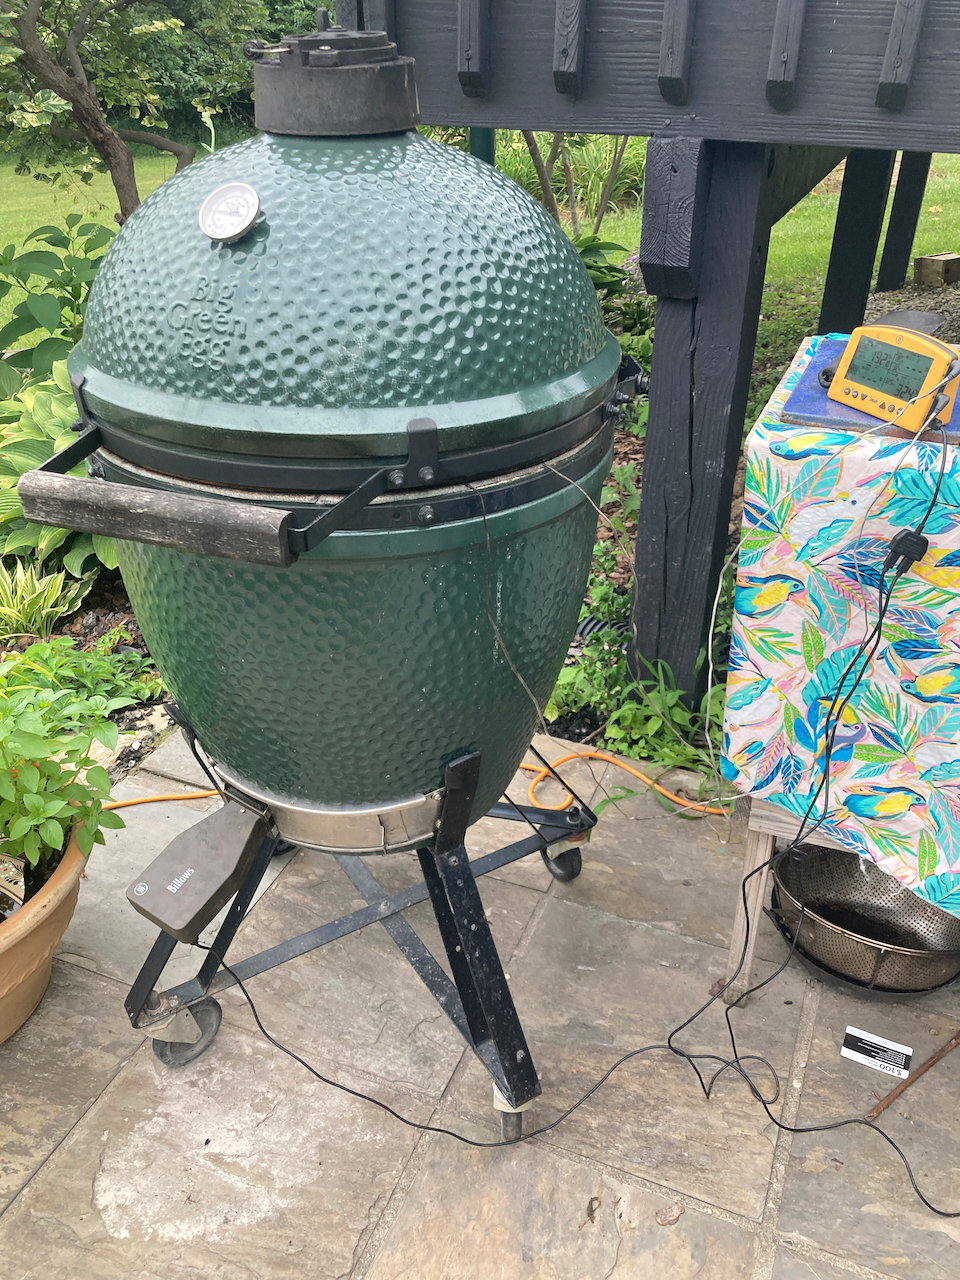
\includegraphics[width=0.7\textwidth,height=\textheight]{images/bgewithbillows.jpeg}

Big Green Egg with Billows and Signals attached.

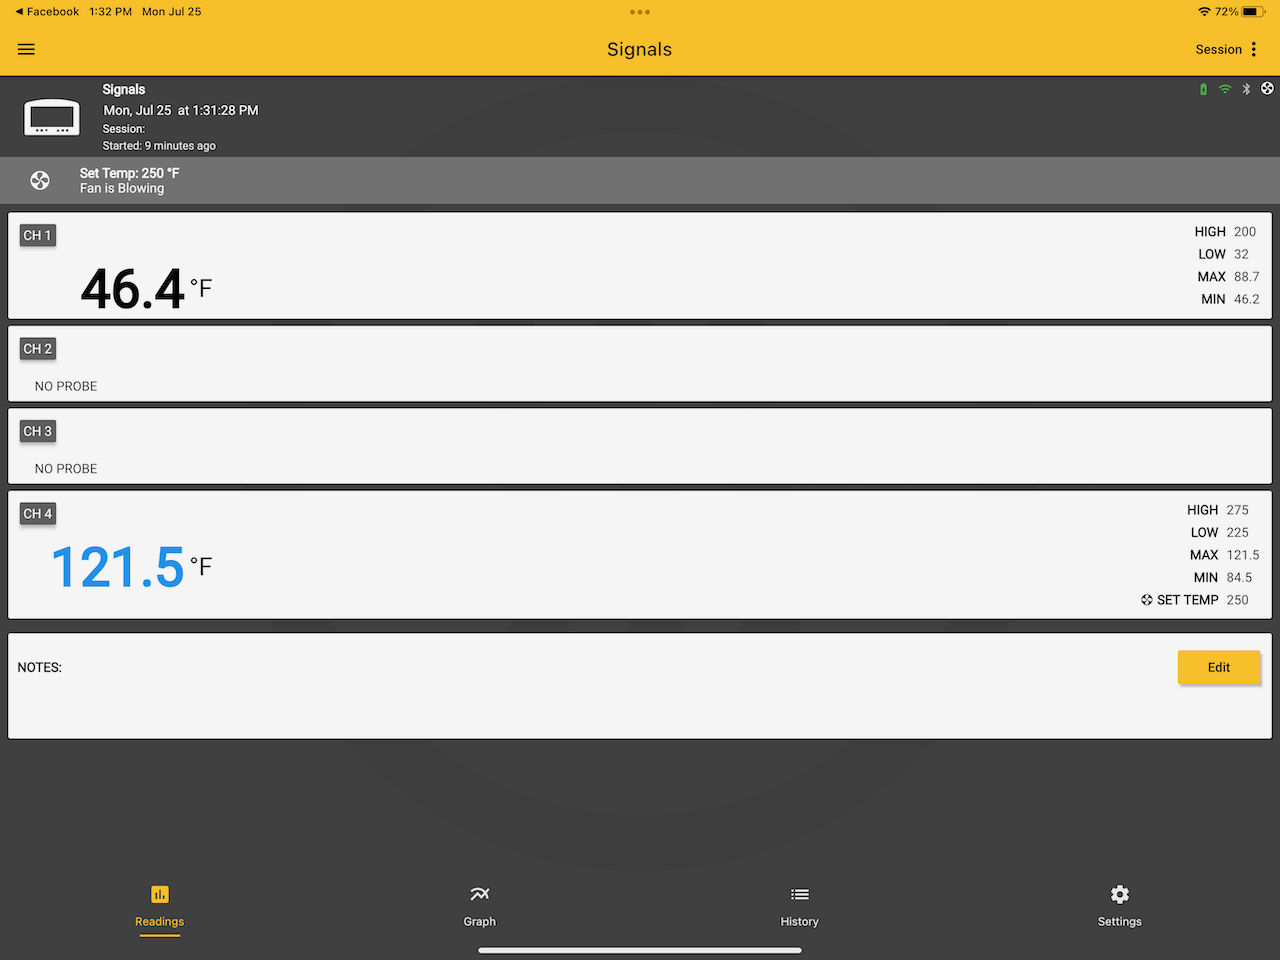
\includegraphics[width=0.4\textwidth,height=\textheight]{images/ThermoScreen.jpeg}~ 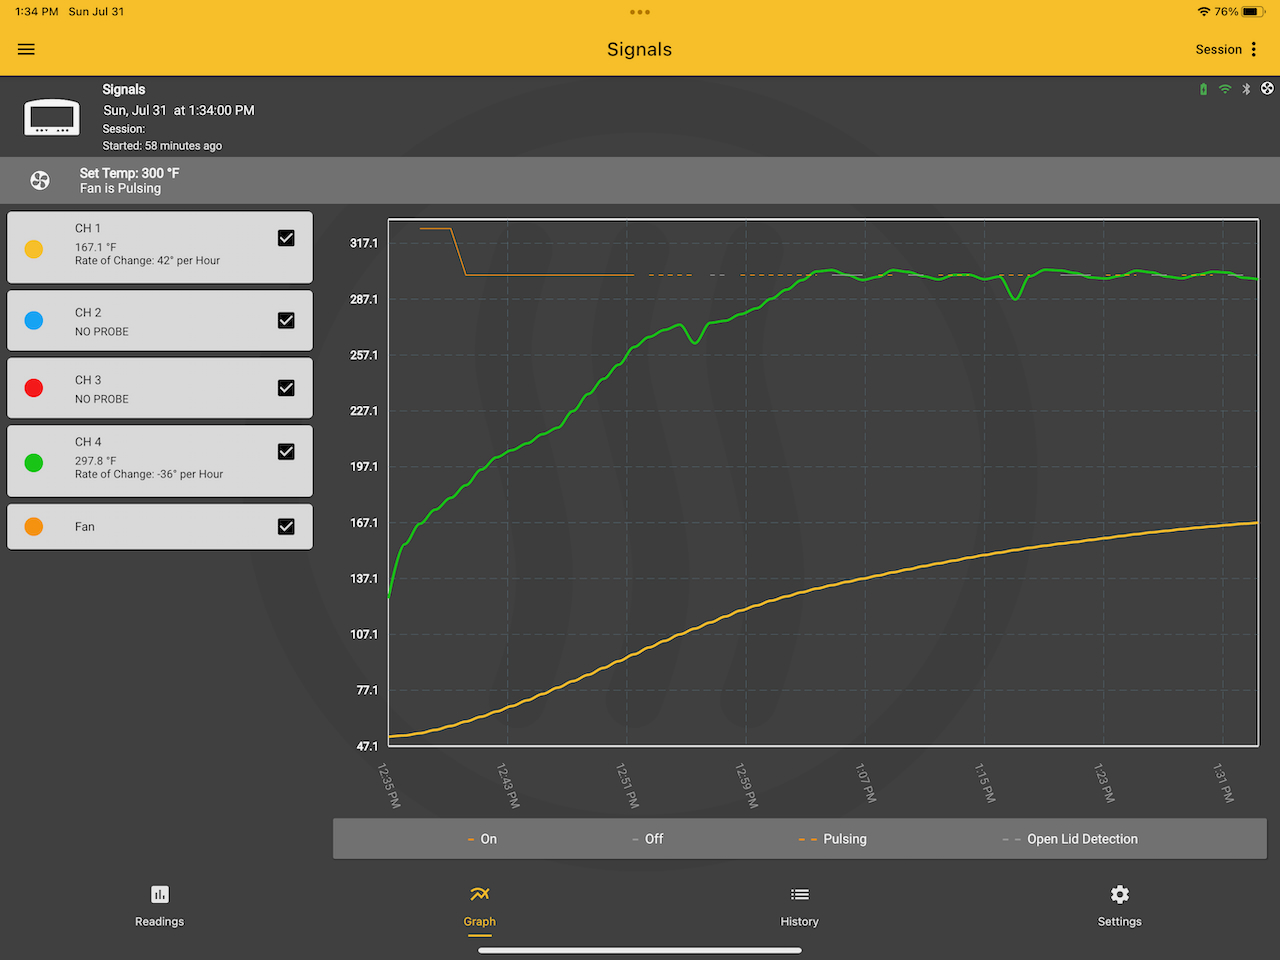
\includegraphics[width=0.4\textwidth,height=\textheight]{images/thermo1hour.jpeg}

Screen shots of Thermoworks app display. Left: Readings screen, showing internal temperature (top) and grill temperature (bottom) at the beginning of a run. Right: Graph screen after one hour of cooking a tritip roast. Grill temperature is in green and internal temperature is in gold.

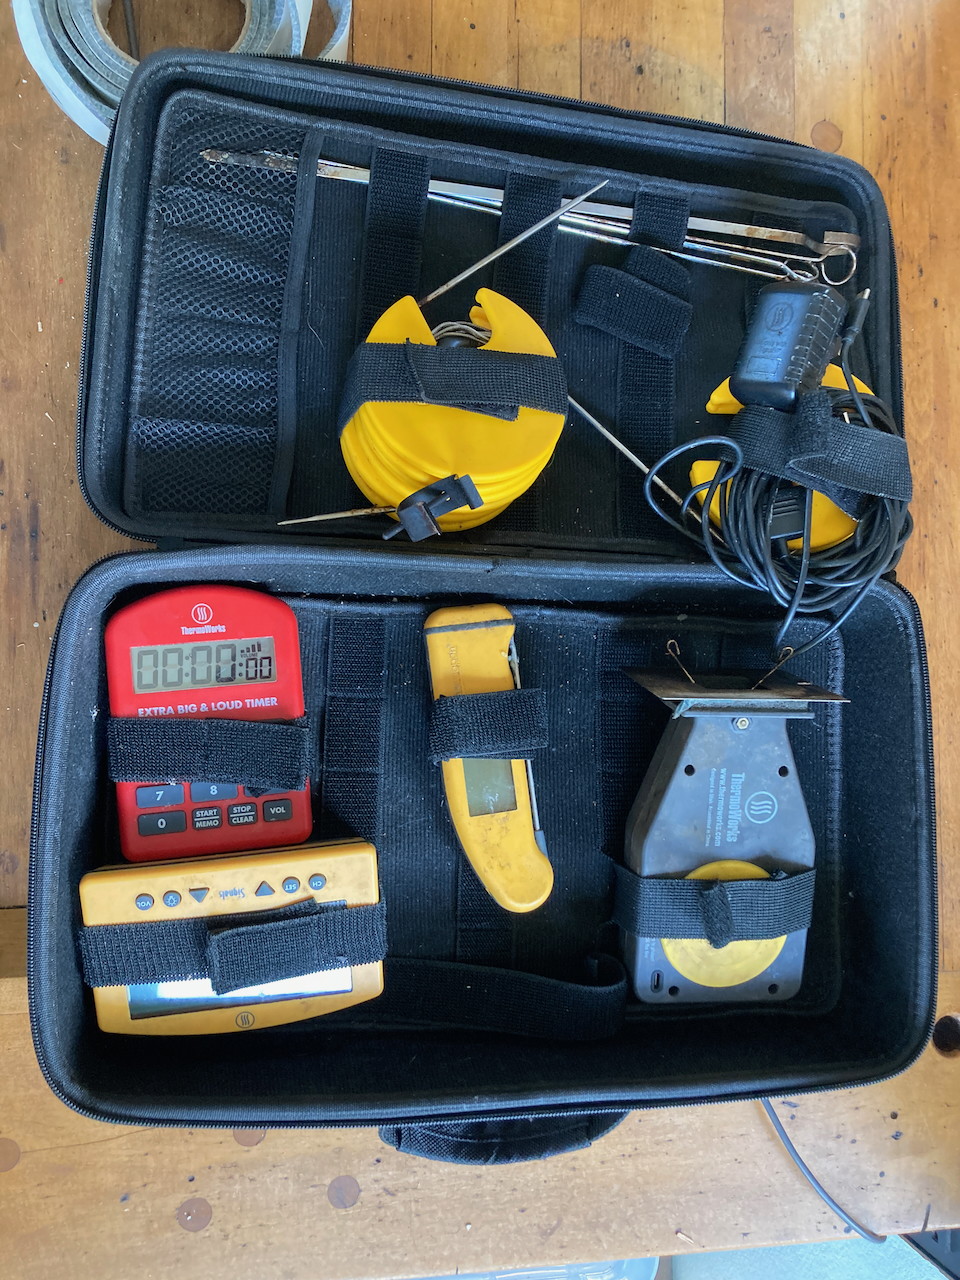
\includegraphics[width=0.7\textwidth,height=\textheight]{images/thermokit.jpeg}

My temperature monitoring and control kit. Clockwise from top: Skewers, wiring for Billows, Billows device, Thermopen, Signals controller, Big and Loud timer.

\hypertarget{grill}{%
\section{Grilling}\label{grill}}

\hypertarget{chicken}{%
\subsection{Chicken}\label{chicken}}

\hypertarget{corn}{%
\subsection{Corn on the cob}\label{corn}}

I am fortunate enough to have grown up in sweet corn country. Indeed, one of my fondest childhood memories is, when we were visiting family friends on a farm in Macedon NY, the children (including me) were sent out in the field to pick fresh corn for the day's dinner. From the field to the pot in 10 minutes - absolutely delicious! Unfortunately, I then spent a big chunk of my life in Florida, and corn there simply doesn't measure up to what I grew up with. Thus, it was absolutely wonder to discover, when I moved to Ohio in July of 2007 (peak corn season) that the corn here measures up to what I remember as a child.

So the first secret about corn on the cob is freshness. Ideally, it should be cooked the day it is picked; with storage, even refrigerated, the sugar in the corn rapidly turns to starch. I have eaten second day corn, which is satisfactory, but fresher is better.

So here's my method for cooking corn on the grill. I'm not sure where I got the original recipe, but it's pretty basic and ubiquitous.

\textbf{Ingredients}

\begin{quote}
2-6 ears of fresh sweet corn, in husks\\
melted butter\\
fresh ground pepper\\
grated parmesan (optional)\\
butcher twine
\end{quote}

\begin{enumerate}
\def\labelenumi{\arabic{enumi}.}
\tightlist
\item
  Peel the husks back (do NOT remove them) and discard silks.
\item
  Place corn into a large kettle of water and let soak for at least an hour.
\item
  Remove the corn from the water, baste with melted butter, and sprinkle with pepper, Parmesan (if desired) and any other flavors you might like (dill is a popular one.
\item
  Cut one \textasciitilde8 inch piece of twine for each ear. Wet them in water to make them easier to tie.
\item
  Fold the husks up over the corn and tie together with twine.
\item
  Place the corn on your grill preheated to 450\textsuperscript{o} and roast a total of 10 minutes, rotating the ears every 2.5 minutes.
\item
  Remove ears from grill. With neoprene mitts on, grasp the ear with one hand and the stem with the other. Snap vigorously and separate the stem and attached husk from the ear of corn (you may want to cut the twine with scissors first).
\item
  Serve with just about anything.
\end{enumerate}

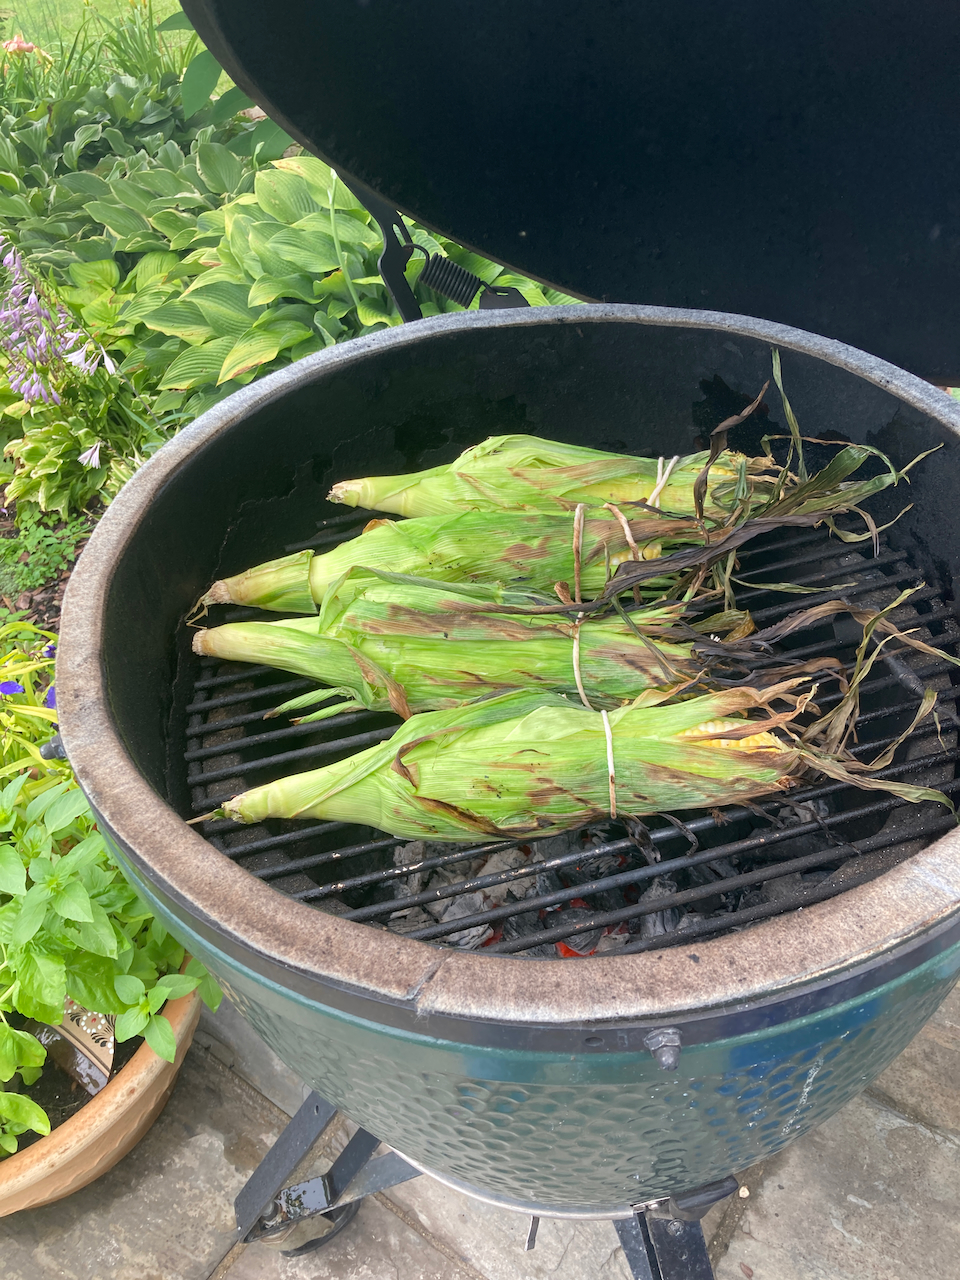
\includegraphics[width=0.5\textwidth,height=\textheight]{images/cornongrill.jpeg}

Corn prepared as described and half way through grilling

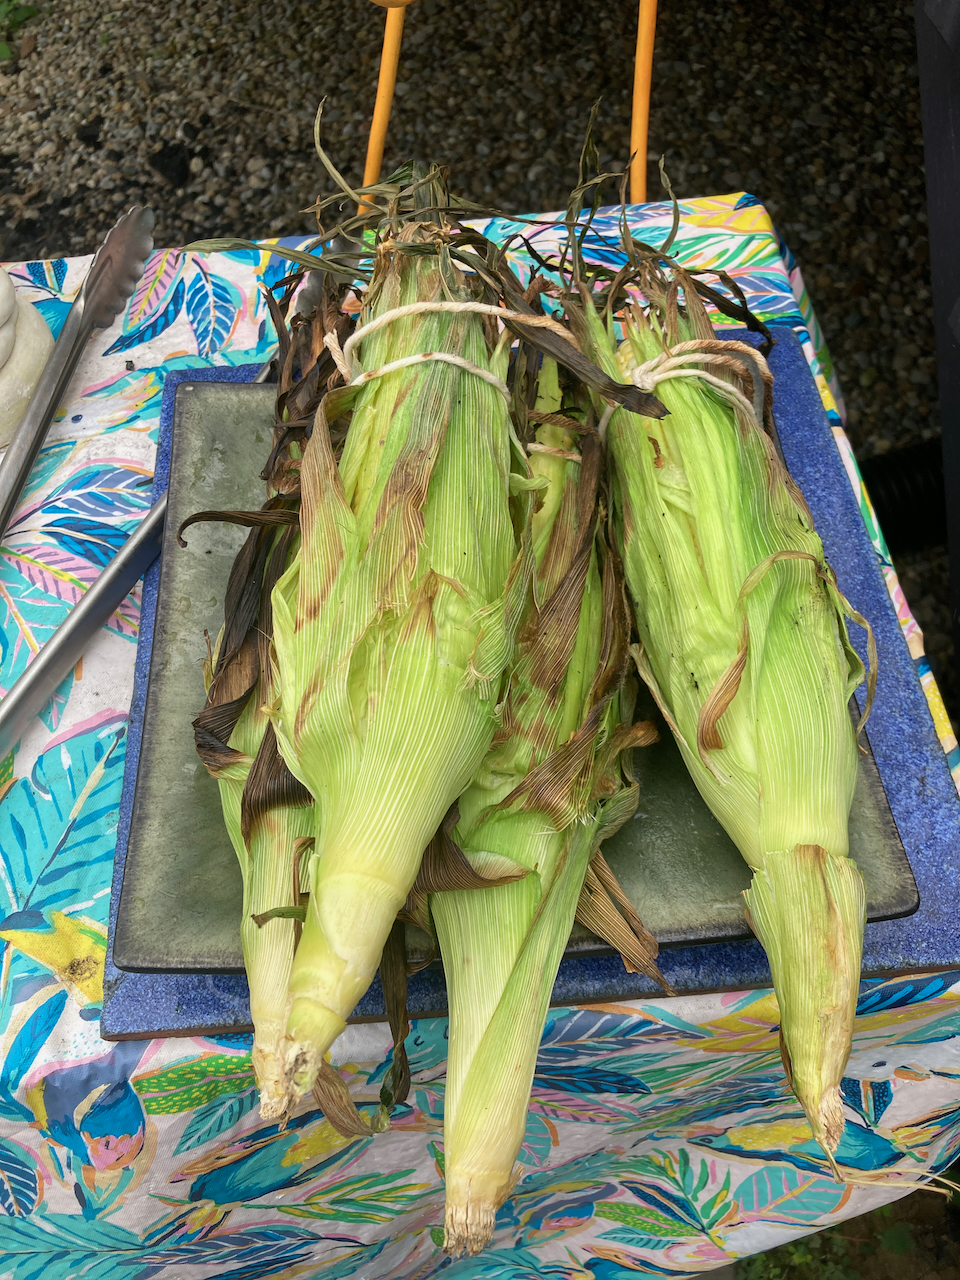
\includegraphics[width=0.5\textwidth,height=\textheight]{images/Corn1.jpeg}

Grilling is complete

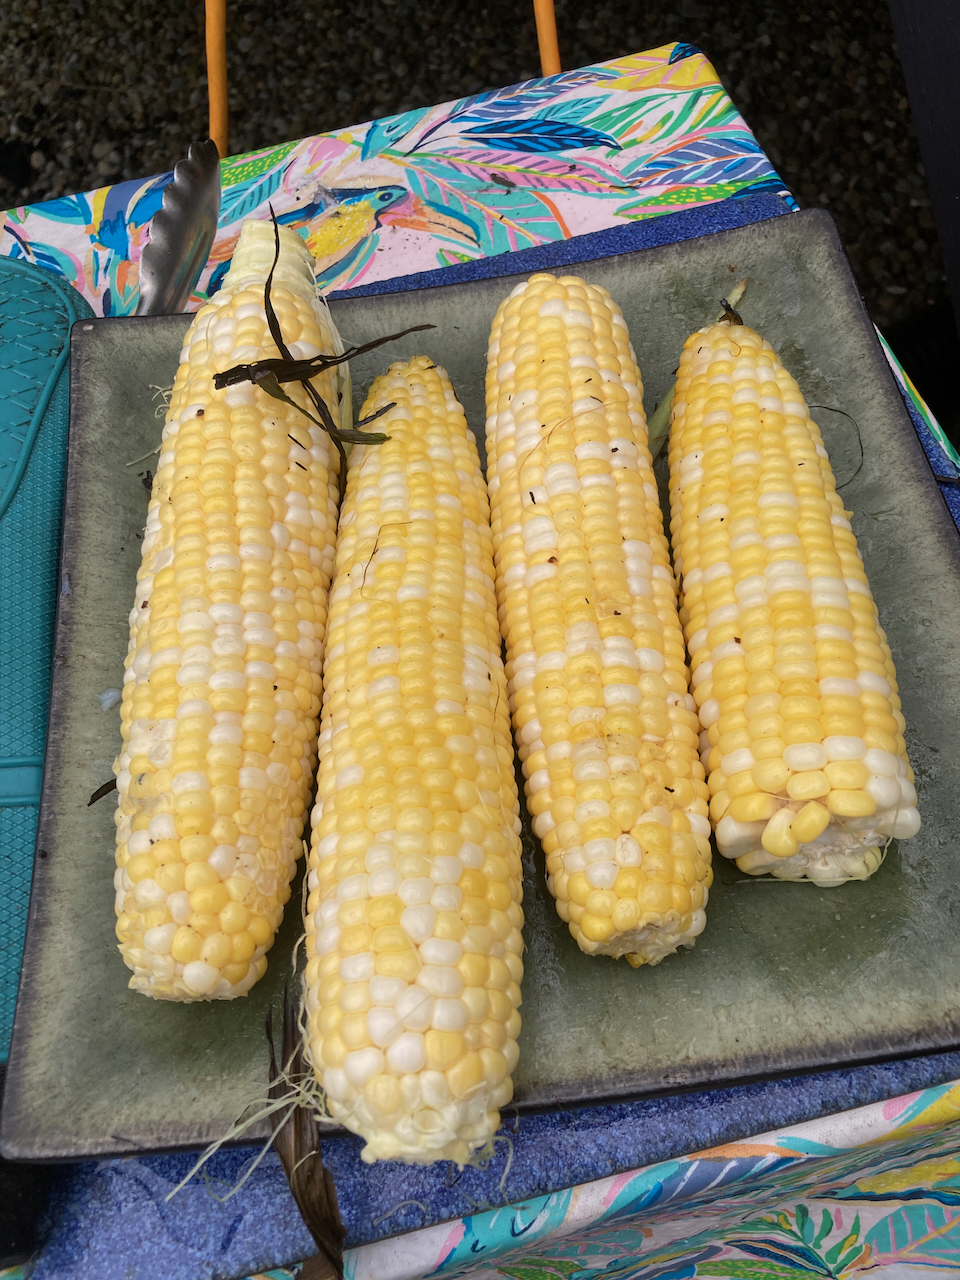
\includegraphics[width=0.5\textwidth,height=\textheight]{images/corn2.jpeg}

Ready to eat

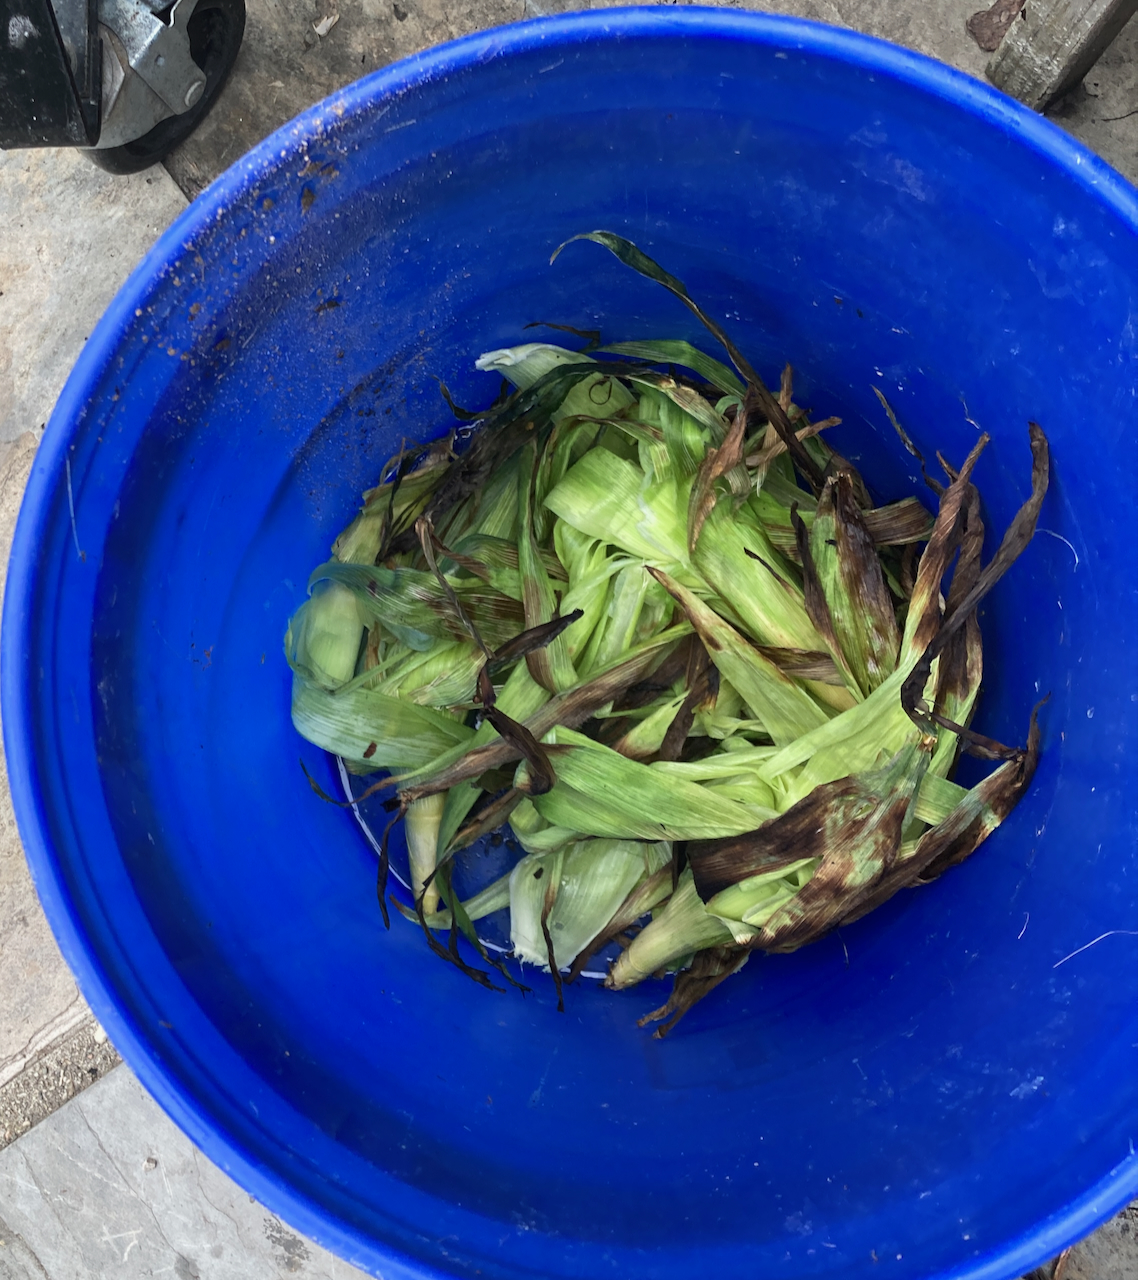
\includegraphics[width=0.5\textwidth,height=\textheight]{images/husks.jpeg}

Ready for the compost pile.

\hypertarget{fajitas}{%
\subsection{Fajitas}\label{fajitas}}

This recipe was originally one designed for the Instant Pot, but it is really easy to prepare it on a grill. It can also be prepared on the stove top, substituting a heavy frying pan for the grill basket.

\textbf{Ingredients}

\begin{quote}
\textasciitilde3/4 lb beef, sliced into strips for stir fry (flank steak works well)\\
2 tbsp fajita seasoning*\\
1 bell pepper\\
1 onion\\
Splash of red wine\\
1 lime, cut into wedges\\
Flour tortillas.
\end{quote}

\begin{enumerate}
\def\labelenumi{\arabic{enumi}.}
\setcounter{enumi}{1}
\tightlist
\item
  Coat the beef with a tablespoon of fajita seasoning and the splash of red wine. Marinate for 30 min to an hour.
\item
  Slice the vegetables and add the remaining sasoning
\item
  Place the meat in a grill basket and cook over a medium hot (450\textsuperscript{o} F.) grill until browned, about 3-5 minutes. Remove and set aside
\item
  Add the vegetables to the basket and cook for about 10 minutes, until vegetables are cooked through.
\item
  Add the meat to the mixture and cook for another 5-10 minutes.
\item
  In your kitchen, briefly warm the tortillas on a frying pan over medium heat. Place in a basket and cover with a kitchen towel.
\item
  Serve the tortillas, filling and lime wedges for people to put together for guests to serve themselves. If desired, add your favorite hot sauce and/or sour cream (not my favorite).
\end{enumerate}

*There are plenty good choices of fajita seasonings out there. If you choose to make your own, here is the \href{https://littlesunnykitchen.com/fajita-seasoning/}{recipe that I use}. If you are an instant pot user, you can find the original recipe \href{https://www.theinstantpottable.com/instant-pot-steak-fajitas/}{here}.

\hypertarget{korean-chicken-skewers}{%
\subsection{Korean Chicken Skewers}\label{korean-chicken-skewers}}

This is another recipe from {[}*Southern Living{]}(and is absolutely delicious and pretty easy to prepare. I cook these on metal skewers that are about 12 inches long and have a flat shape, so that the skewered food is easier to handle.

\textbf{Ingredients}

\begin{quote}
1/2 cup unsalted butter\\
2 garlic cloves, peeled and grated\\
1/3 cup honey
1 tsp kosher salt
1 tsp rice vinegar\\
2 lb boneless skinless thighs, cut into 1 inch cubes\\
1 large red onion, cut into wedges
\end{quote}

\begin{enumerate}
\def\labelenumi{\arabic{enumi}.}
\tightlist
\item
  Prepare your grill for direct cooking at 450\textsuperscript{o} F,
\item
  Melt the butter on the stovetop over medium low heat.\\
\item
  Add the garlic and cook for about two minutes.
\item
  Add the salt, vinegar and 2 Tbsp soy sauce, bring to a boil, and cook for about 2 minutes.\\
\item
  Toss the chicken with the remaining soy sauce.
\item
  Thread the chicken and onion wedges onto skewers, adding two pieces of chicken followed by one onion wedge.
\item
  Grill, basting often with honey butter mixture, for 10-12 minutes until chicken is light charred and cooked (if you want to check with an instant read thermometer, the internal temperature of the chicken should be \textasciitilde165\textsuperscript{o}.
\item
  Serve over rice or bucatini.
\end{enumerate}

\hypertarget{bbq}{%
\section{Barbecuing}\label{bbq}}

\hypertarget{some-basics}{%
\subsection{Some Basics}\label{some-basics}}

\hypertarget{beef-and-pork}{%
\subsection{Beef and Pork}\label{beef-and-pork}}

\hypertarget{tritip}{%
\subsubsection{\texorpdfstring{\href{https://blog.thermoworks.com/beef/brisket-style-tri-tip/}{Brisket Style Tritip}}{Brisket Style Tritip}}\label{tritip}}

This is a great place to start in your barbecue adventure. Unlike a brisket, it is a small piece of meat, more suitable for 1-2 people (although it will yield up multuple servings. Furthermore, the cook time is reasonable (6-7 hours), and leftovers will keep in the refrigerator for days.

Ingredients:

\begin{quote}
2-3 pound Tri-tip roast\\
Your favorite beef barbecue rub (I use \href{https://www.penzeys.com/online-catalog/bbq-3000/c-24/p-327/pd-s}{Penzey's Barbecue 3000}\\
3-4 Oak or Hickory Wood Chunks\\
Orange Butcher paper (available at \href{http://www.lowes.com}{Lowes})
\end{quote}

\begin{enumerate}
\def\labelenumi{\arabic{enumi}.}
\tightlist
\item
  Soak the wood chunks in water for at least 30 minutes.
\item
  Load the barbecue with charcoal and add two Fire Starter Sticks. Ignite.
\item
  As soon as the flame dies down, add the soaked wood chips and stir them into the coals as best you can.
\item
  Place your ConvEGGtor, and aluminum drip pan, and grill in place
\item
  \emph{Immediately} hook up your Billows device with a long probe in channel 1 and your grill monitoring probe (attached to the grill).\\
\item
  Using the Thermoworks app, set the fan temperature to 250\textsuperscript{o} F. Close the upper vent on the Egg nearly completely
\item
  Apply a binder to the tri-tip. Mustard is the standard here, however I use olive oil.
\item
  Apply rub liberally to all sides
\item
  Insert a long probe into the heart of the roast and place on grill. Close the lid and let the cooking commence.
\end{enumerate}

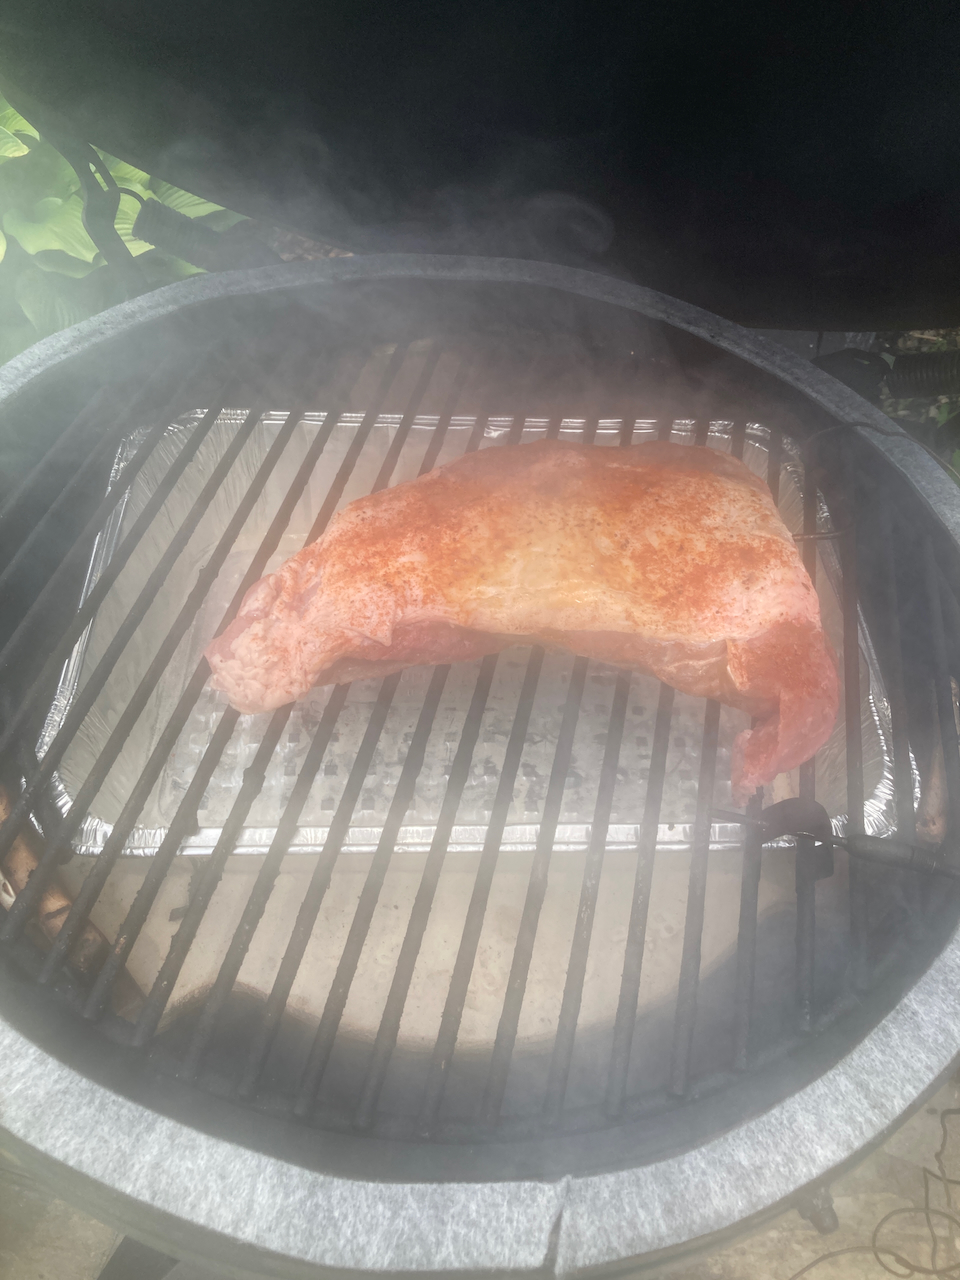
\includegraphics[width=0.4\textwidth,height=\textheight]{images/tritip1.jpeg}~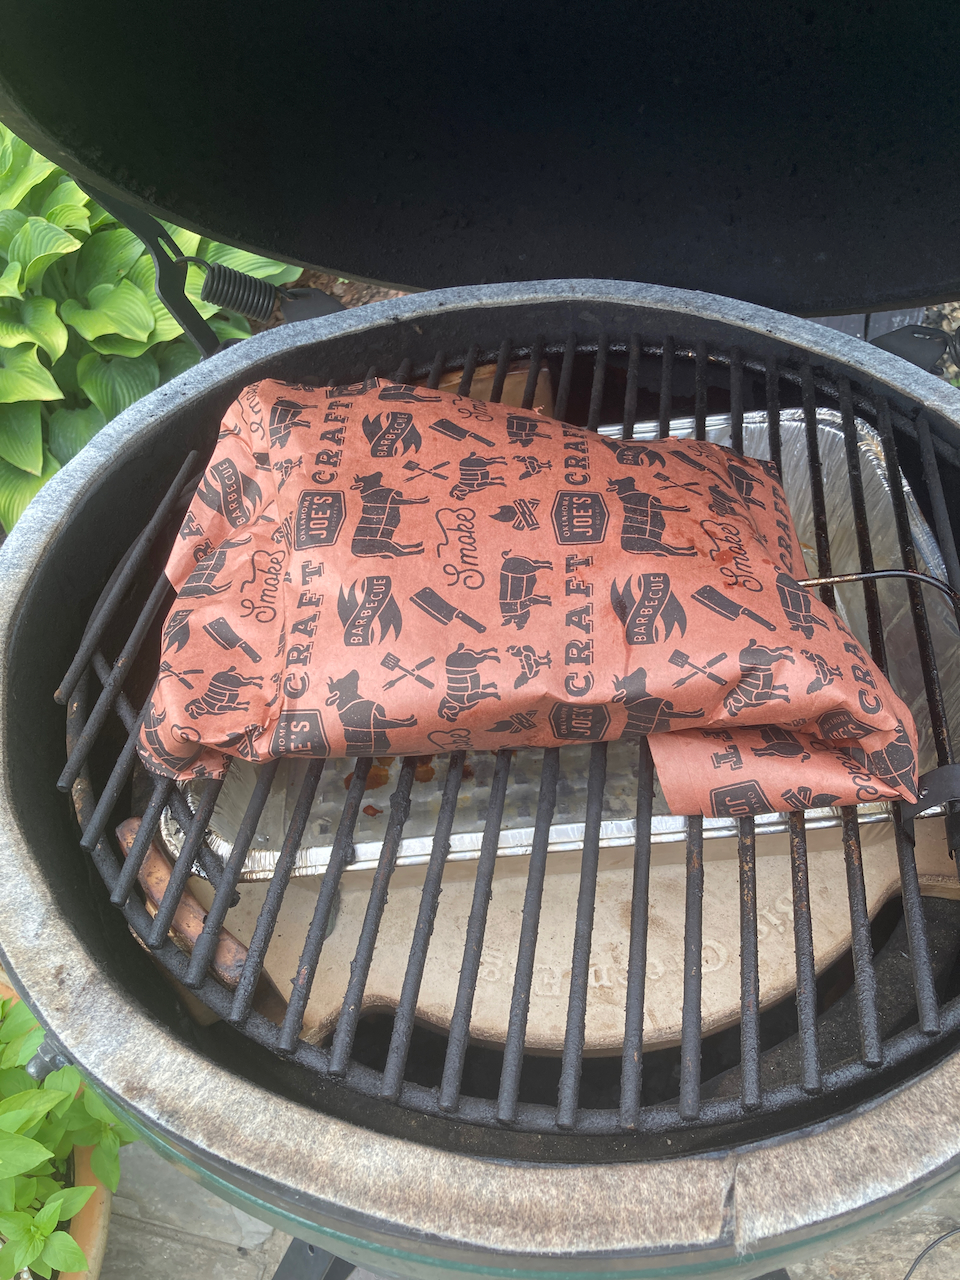
\includegraphics[width=0.4\textwidth,height=\textheight]{images/tritipwrapped.jpeg}

Left: Beginning the barbecue Right: Tritip wrapped in butcher paper for final cook.

At this point, sit back, have a beer or a glass of wine, and keep an eye on time and temperature. When the internal temperature reaches 150\textsuperscript{o} F. or when 2 hours have past (whichever comes first), proceed as follows:

\begin{enumerate}
\def\labelenumi{\arabic{enumi}.}
\tightlist
\item
  Remove the roast from the Egg, keeping lid-open time to a minimum.
\item
  Wrap the roast in two layers of orange butcher paper.
\item
  Return the roast to the Egg, and with the app, increase the grill temperature to 275\textsuperscript{o} F.
\item
  When the roast has reached 200\textsuperscript{o} F. (about 3-4 hours), remove it and let it stand wrapped for 20 minutes or so.
\item
  Slice and enjoy!
\end{enumerate}

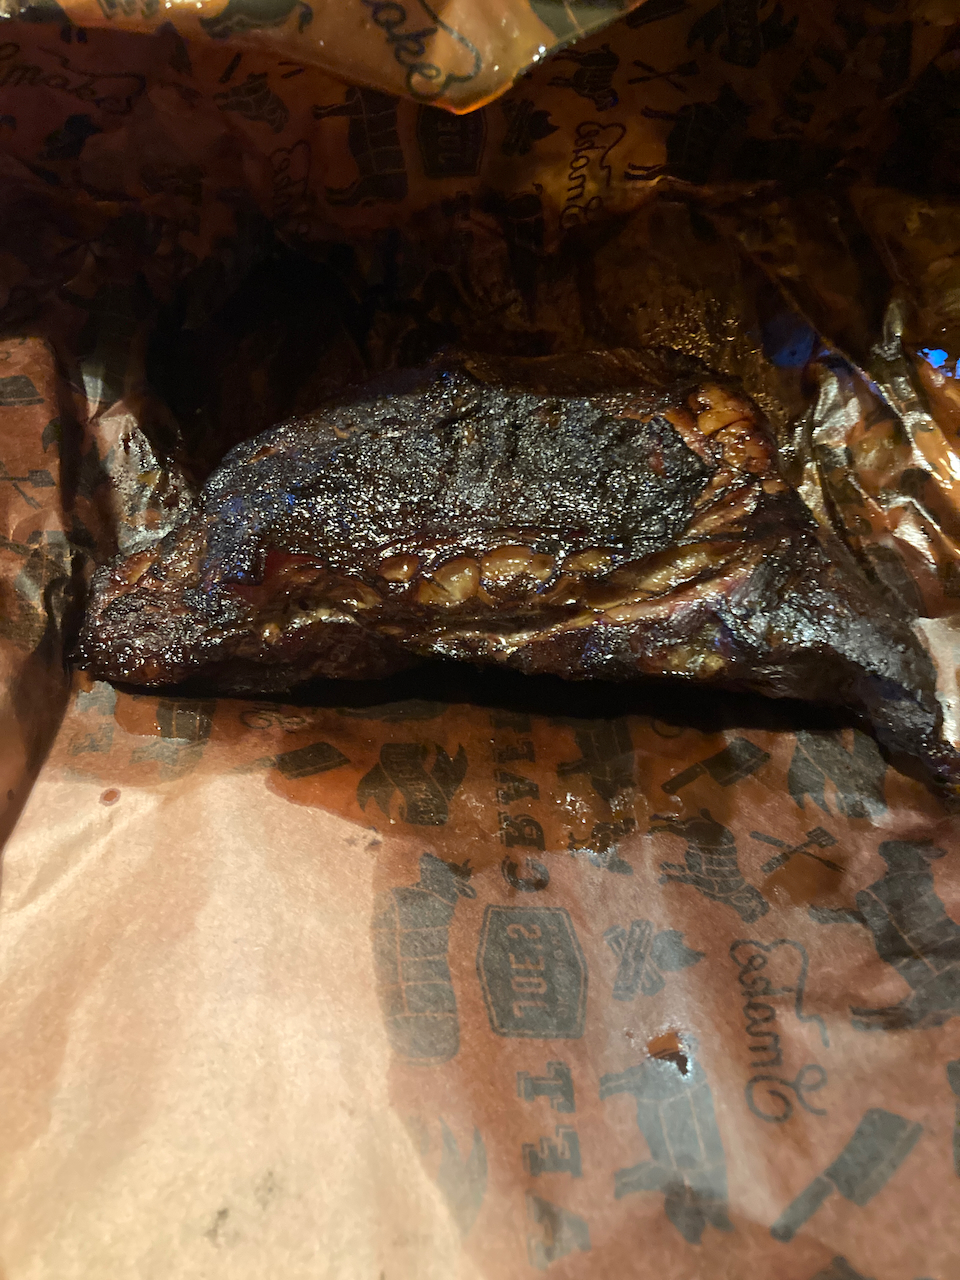
\includegraphics[width=0.4\textwidth,height=\textheight]{images/tritipafter1.jpeg}~ 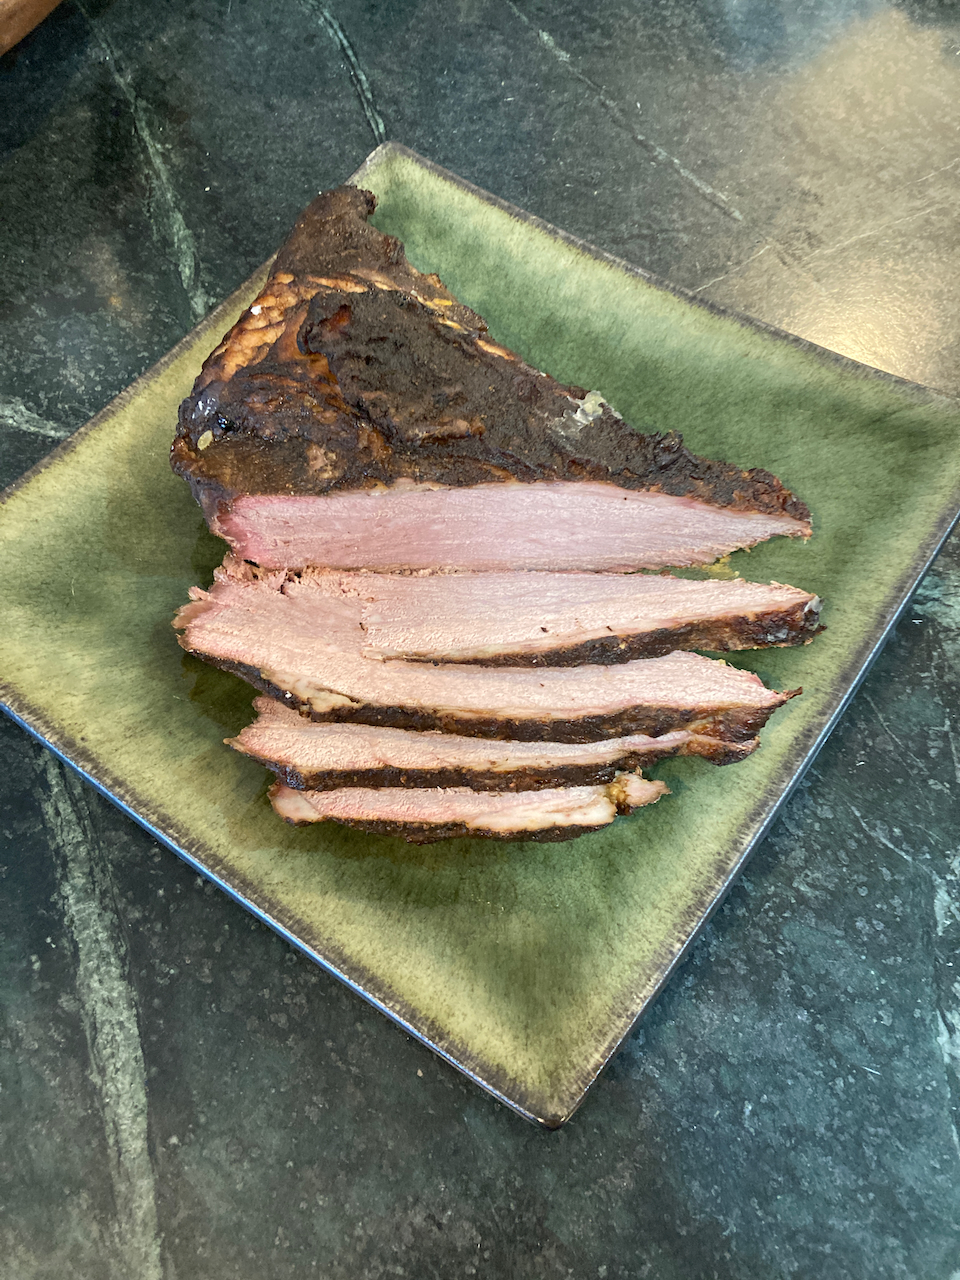
\includegraphics[width=0.4\textwidth,height=\textheight]{images/tritipafter2.jpeg}

Cooked and sliced.

\hypertarget{roast-beef-for-sandwiches}{%
\subsubsection{Roast beef for sandwiches}\label{roast-beef-for-sandwiches}}

This is one that showed up in my inbox from \href{https://blog.thermoworks.com/blog/homemade-deli-style-roast-beef/}{Thermoworks}. I haven't tried it yet, but I'm betting it will work well barbecued on the grill. Note that the original recipe calls for a preliminary sear; I'm betting that smoking without the convEGGtor will get the job done.

\textbf{Ingredients}

\begin{quote}
1 eye round roast, 2-3 lb\\
kosher salt\\
black pepper
\end{quote}

\begin{enumerate}
\def\labelenumi{\arabic{enumi}.}
\tightlist
\item
  The night before you cook, salt the roast generously and place in the refrigerator covered.
\item
  Prepare your grill for low temperature smoking at 200\textsuperscript{o}. You may or may not want to add wood chunks (oak or hickory).
\item
  Rinse off excess salt, dry, and apply pepper.
\item
  Barbecue at 200\textsuperscript{o} F until internal temperature reaches 120-130\textsuperscript{o} F. (lower for more rare meat, higher for more tender).
\item
  Use your instant read thermometer to check for doneness.
\item
  For ease of slicing, put roast in the refrigerator overnight.
\end{enumerate}

\hypertarget{pig-wings}{%
\subsubsection{\texorpdfstring{\href{https://blog.thermoworks.com/bbq-grilling/pig-wings/}{Pig Wings}}{Pig Wings}}\label{pig-wings}}

Despite the fact that we live near Cincinnati, home of the Flying Pig Marathon, these are not made from avian porcines. Rather, they are partially deboned and trimmed pork shanks, prepared with a sauce similar to traditional buffalo wing sauce. The meat may be available from a local butcher shop; online it can be had at \href{https://porterroad.com/}{Porter Road} in Nashville (a great source of meat, but expensive, with high shipping costs). Alternatively, you may be able to get properly trimmed pork shanks from your local butcher shop.

Like brisket or pork butt, shanks are full of connective tissue that must be broken down in order to yield a properly tender result. This will occur if the meat is cooked to an internal temperature of 200\textsuperscript{o} F. That processed is hastened by covering the pan containing ``wings'' and sauce for the second half of the cooking.

\emph{Ingredients}

\begin{quote}
Pig wings (however many you want)\\
BBQ rub\\
1 onion, sliced or diced.\\
8 oz. butter\\
8 oz. hot sauce (your favorite)\\
Juice of half a lemon\\
1 tbsp. mustard powder\\
1/2 cup apple cider vinegar\\
12 oz. beer
\end{quote}

\begin{enumerate}
\def\labelenumi{\arabic{enumi}.}
\tightlist
\item
  Prepare your smoker as you did for \protect\hyperlink{tritip}{tri-tip}. For this recipe, you want to reach a cooking temperature of 250\textsuperscript{o} F. Hickory or apple wood work well for this recipe.\\
\item
  Remove any excess fat and the silver skin (if any) from the wings.
\item
  Season with BBQ rub (or with salt, pepper and garlic powder).
\item
  Place in the smoker and cook for 1 hour, turning every 20 minutes.
\item
  While the wings are smoking, make the sauce as follows:

  \begin{enumerate}
  \def\labelenumii{\alph{enumii}.}
  \tightlist
  \item
    Melt the butter, add the onion, and sauté until soft.\\
  \item
    Add all of the remaining ingredients EXCEPT the beer and let it boil for a couple of minutes.\\
  \item
    Add the beer and boil for an additional 5 minutes.
  \end{enumerate}
\item
  After the hour of cooking above, mop the wings with the sauce. Continue to cook for an additional hour or until the internal temperature reaches 180\textsuperscript{o}, mopping every 20 minutes or so.
\item
  Transfer the wings to an aluminum pan with \textasciitilde1/2 inch of sauce in it. Top the wings with some of the onions from the sauce.
\item
  Cover the pan with foil, insert an internal temperature probe into one of the wings through the foil.
\item
  Cook until the internal temperature reaches 200\textsuperscript{o}. Verify with your instant read thermometer.
\item
  Allow wings to rest 10-15 minutes and then serve.
\end{enumerate}

\hypertarget{poultry}{%
\subsection{Poultry}\label{poultry}}

\hypertarget{chicken-wings}{%
\subsubsection{Chicken Wings}\label{chicken-wings}}

What's not to love about chicken wings? Aside from the fact that they are messy to eat, they are very tasty, either by themselves or (as is more common) dipped in one of many different wing sauces. Of course, wings are often broiled or fryed, but I have found that slow cookin on the barbecue works very well. My preference is for wings that have been sectioned prior to cooking, but that is not necessary if you prefer keeping them whole.

\textbf{Ingredients}

\begin{quote}
2 lb. chicken wings\\
barbecue seasoning of choice (salt and pepper would also work)\\
4 oz. hot sauce,*\\
3 tbsp. butter
\end{quote}

\begin{enumerate}
\def\labelenumi{\arabic{enumi}.}
\tightlist
\item
  Prepare your grill for smoking at 220\textsuperscript{o}F. I do not use wood chunks for this - the charcoal imparts plenty of flavor.
\item
  Pat the wings dry with paper towels, and if sectioning, use game shears to separate the tips, flats, and drumettes. Discard the tips (or save them for making stock).
\item
  Liberally apply rub.
\item
  Place the wings on the grill, with a short needle probe inserted into the largest piece. If you have a grilling rack (see photo below), use it.
\item
  When the internal temperature reaches 125\textsuperscript{o} F., turn the wings over.
\item
  While they are continuing to cook, melt the butter and stir in the hot sauce.
\item
  When the internal temperature reaches 165\textsuperscript{o}, remove the wings, stir in with the hot sauce mix, and serve.
\end{enumerate}

* Given my western New York heritage, I am partial to Buffalo style wings. Of course there are hundreds of commercial sauces available; I actually use one I get from an Amish market in Adams County Ohio. A more widely available alternative is \href{https://www.tabasco.com/hot-sauces/buffalo-style-hot-sauce/}{Tabasco Bufalo Style Hot Sauce}. Alternatively there are lots of recipes for making your own, either Buffalo style or your favorite alternative. One that I like is \href{https://www.tabasco.com/hot-sauces/buffalo-style-hot-sauce/}{Korean barbecue ribs} published recently in \emph{Southern Living}:

\begin{quote}
1/2 cup gochujang (available in the Asian section of most food stores or at specialty markets)\\
2 tbsp sesame oil\\
2 tbsp honey\\
1 tbsp peeled and grated ginger
3 cloves garlic, peeled and chopped
chopped scallions\\
toasted sesame seeds.
\end{quote}

The recipe given calls for the wings to be marinated in the first five ingredients for an hour, after which they are cooked as described above. I'm sure this mix would also work if the wings were to be dipped in it after cooking rather than before. Either way, the scallions and sesame seeds are sprinkled on the cooked wings before serving.

\hypertarget{fish}{%
\subsection{Fish}\label{fish}}

\hypertarget{comfort}{%
\chapter{``Comfort'' Food}\label{comfort}}

So now we come to what might be called ``What do I do in winter?'' section. In fact, living here in southern Ohio, I can now count on at least a few barbecue days every month of the year. But of course there are many days when that is not possible. So, having to retreat indoors, I use a collection of recipes, many derived from my pre-Green Egg days, that yield excellent results using the stovetop, oven, and microwave. In many cases, since I am preparing only 1-2 servings, I can use our toaster oven instead of our lovely Big Chill range.

\hypertarget{chicken-1}{%
\section{Chicken}\label{chicken-1}}

\hypertarget{lemon-chicken}{%
\subsection{Lemon Chicken}\label{lemon-chicken}}

This recipe is derived from a 40 year old cookbook - \emph{The Silver Palate Cookbook} by Julee Rosso and Sheila Lukins. At the time of publication, the authors ran a small restaurant in New York City; since then they have expanded to \href{https://www.silverpalate.com/}{the web}, where you can find an extensive selection of sauces and recipes. Some of their products may be available at a \href{https://www.silverpalate.com/stores}{store near you}.

Note that the big difference between the original recipe and mine is that the chicken is initially broiled rather than fried. This was a technique suggested by my late sister Nancy Cochrane, someone who abhorred grease in cooking. That is indeed true - the results I typically obtain after the broiling are dry and crisp (the chicken will be well moistened in the subsequent baking). Also, I've provided what I use for two servings of dark meat, but it can can easily be scaled up or down, and white meat can be used if preferred.

Ingredients:

\begin{quote}
4 Bone-in chicken thighs\\
White flour (about 1/3 cup)\\
1 tsp. ground black pepper\\
1 tsp. paprika (I use Penzey's \href{https://www.penzeys.com/online-catalog/hungarian-style-half-sharp-paprika/c-24/p-1147/pd-s}{Hungarian Half Sharp}, but feel free to use your favorite)\\
1 lemon\\
brown sugar\\
1/3 cup chicken broth
\end{quote}

\begin{enumerate}
\def\labelenumi{\arabic{enumi}.}
\tightlist
\item
  Combine the flour, pepper and paprika in a plastic bag.
\item
  Zest the lemon and then slice it as thinly as possible.\\
\item
  Add the chicken pieces one at a time to the bag and make sure they are coated evenly with the flour mix.
\item
  Place chicken into a baking dish (a 7 X 11 glass one works fine) skin side up and broil, watching regularly, until the chicken is lightly browned. Flip the chicken over and do the same with the other side
\item
  Set the oven to bake at 375\textsuperscript{o}. Sprinkle the lemon set and brown sugar evenly over the top of the chicken pieces. Pour the broth into the dish (not over the chicken).
\item
  Bake at 375\textsuperscript{o} for 35-40 minutes.
\end{enumerate}

Feel free to be creative in how you serve; I usually have this with white rice and a side of applesauce.

\hypertarget{berberecurry-chicken}{%
\subsection{\texorpdfstring{\href{https://www.penzeys.com/shop/recipes/berbere-chicken-and-rice/}{Berbere/curry chicken}}{Berbere/curry chicken}}\label{berberecurry-chicken}}

This one is lifted straight from the Penzey's web - it's been tweaked a little and adapted for slow cooking.The biggest change I made was to double the amount of Curry and Berbere seasoning, rendering the dish spicier. For firmer chicken, cook on the stove top; rather than 3 hours of slow cooking, cook for \textasciitilde45 minutes over medium low heat.

\begin{quote}
6 boneless skinless chicken thighs, cubed\\
1 tbsp olive oil\\
1 small red onion, chopped coursely\\
\textasciitilde{} 2 tsp curry powder (I use Penzey's {[}Now Curry{]}\\
\textasciitilde2 tbsp Penzey's \href{https://www.penzeys.com/online-catalog/berbere-seasoning-blend/c-24/p-155/pd-s}{Berbere Seasoning}\\
1 14.5 oz. can diced tomatoes, drained
\end{quote}

\begin{enumerate}
\def\labelenumi{\arabic{enumi}.}
\tightlist
\item
  Use the sauté setting to heat the oil, and add the onions, stirring occasionally, until they are softened (about 10 minutes).\\
\item
  Add the chicken and cook, stirring as needed, until it is browned (5-8 minutes).\\
\item
  Add the two spices and stir
\item
  Add the tomatoes, cover, and slow cook on high for 3 hours (or over medium to low heat for 45 minutes to an hour).
\item
  If necessary, uncover and set the heat to sauté to reduce the sauce. Serve over white rice.
\end{enumerate}

\hypertarget{cacciatore}{%
\subsection{Chicken Cacciatore}\label{cacciatore}}

This is one of the very few recipes that I concocted by myself - I don't really even remember when. For convenience sake, I usually do it in our slow cooker, but it can also be done (in less time) on the stove top. I've included the slow cooker instructions below, with parenthetical notes about doing it on the stove top.

Ingredients:

\begin{quote}
1-2 tbsp olive oil
2 lb. boneless chicken thighs, cut into 1 inch cubes (white meat can be substituted if you prefer)\\
1 red onion, chopped\\
2-3 cloves garlic, chopped\\
1 bell pepper, chopped\\
1 14.5 oz can diced tomatoes, drainged\\
1/2 cup red wine
1 tbsp. red wine vinegar\\
1/4 - 1/2 tsp crushed red pepper\\
1 tsp black pepper\\
2 tsp \href{https://www.penzeys.com/online-catalog/italian-herb-mix/c-24/p-183/pd-s}{Penzey's Italian Herb Mix} (a mix of dried basil and oregano can be substituted)
\end{quote}

\begin{enumerate}
\def\labelenumi{\arabic{enumi}.}
\tightlist
\item
  Set the slow cooker to sauté and add the olive oil and onions. Sauté for 10 minutes until onions or soft (alternatively, do this in a metal casserole over medium heat on your stove).\\
\item
  Add the garlic and bell pepper and cook for 5 more minutes.
\item
  Add the chicken and cook, stirring, until it is browned (5-8 minutes).\\
\item
  Add the tomatoes, wine, crushed red pepper, black pepper and Italian seasoning to the mix*
\item
  Set the slow cooker on ``slow cook - high'', cover, and let it cook for 3 hours (On the stove top, reduce heat to medium low, cover, and cook for 45 minutes to an hour)
\item
  Uncover the pot. If the liquid needs reducing, return the slow cooker to sauté and cook until the desired consistency is achieved (on the stove top, raise heat to medium and do the same).
\item
  Serve over white rice or pastas
\end{enumerate}

\begin{quote}
* In actuality I don't usually measure the spices - I just sprinkle them on as I see fit. Thus, you should consider the amounts given as approximations and fee free to adjust them to taste. Furthermore, if you have an Italian herb blend you like, feel free to use it.
\end{quote}

\hypertarget{comeat}{%
\section{Pork and beef}\label{comeat}}

\hypertarget{raging-rigatoni}{%
\subsection{``Raging'' Rigatoni}\label{raging-rigatoni}}

This is another old one, dating back (for me) to the 1970's and is derived from \emph{The Complete Book of Pasta}, by Jack Denton Scott. A more formal name for it is Rigatoni All'Arrabbiatta. It is simple to make, and leftovers reheat well. The biggest change I made was to add onions and garlic to it. I also do not saute the bacon; rather I let it cook with the sauce, resulting in what I think is a much more flavorful dish.

\textbf{Ingredients}

1 tbsp. olive oil\\
1 small onion, coarsely sliced\\
2 garlic gloves, grated\\
4 slices bacon\\
2-3 jalapeno peppers, sliced\\
1 28 oz can tomatoes (San Marzano are the best, but any will work)\\
Italian seasoning and black pepper to taste\\
6-8 oz pasta (the original calls for rigatoni, but I often substitute penné, ziti, or some other similar tube variety)\\
grated parmesan or romano cheese

\begin{enumerate}
\def\labelenumi{\arabic{enumi}.}
\tightlist
\item
  Sauté onions and garlic in oil until soft in a 12 inch skillet, about 5-10 minutes
\item
  Add tomatoes, bacon, peppers and seasoning.
\item
  Cook uncovered over medium heat for about 15 minutes, stirring occasionally with a spatula, chopping the tomatoes and breaking apart the bacon as you do so.
\item
  Cook uncovered over medium heat for about 15 minutes, stirring occasionally with a spatula, chopping the tomatoes as you do so.
\item
  While the sauce is reducing, cook your pasta by your favorite method (I use water with a dash of olive oil) *al denté and drain.
\item
  Combine the sauce and the pasta and serve, with parmesan or romano cheese available to sprinkle over servings.
\end{enumerate}

Like all Italian food, this goes well with a serving of crusty bread (like \protect\hyperlink{baguettes}{baguettes} and a side salad.

\hypertarget{coseafood}{%
\section{Seafood}\label{coseafood}}

\hypertarget{shrimp-in-red-sauce}{%
\subsection{Shrimp in red sauce}\label{shrimp-in-red-sauce}}

When possible, I really prefer grilling shrimp, but when that is impossible, here's a recipe I like to use. It comes from \emph{Italian}, by Whiteman, Wright and Boggiano, a book I picked up in a bargain bin a long time back. Note that the sauce is somewhat similar to my recipe for \protect\hyperlink{cacciatore}{chicken cacciatore}, and it can be used as a basic red sauce as desired (it works well as a pizza sauce or by itself over pasta).

\begin{quote}
1/2 to 3/4 lb. shrimp, peeled and de-veined
\end{quote}

\hypertarget{panko-encrusted-baked-fish}{%
\subsection{Panko-encrusted baked fish}\label{panko-encrusted-baked-fish}}

\hypertarget{conomeat}{%
\section{Non-meat and -fish}\label{conomeat}}

\hypertarget{macaroni-and-cheese}{%
\subsection{Macaroni and cheese}\label{macaroni-and-cheese}}

This is an old classic of mine, one that I developed in the 1970's. As I noted earlier, it was derived from a recipe for cheese sauce in \emph{The Joy of Cooking}; I have changed the cheese mix, livened up the spicing, and incorporated use of my microwave oven into the preparation.

\textbf{Ingredients}

3 tbsp. butter\\
2 tbsp flour\\
1 cup whole milk\\
1/2 tbsp dry mustard\\
1/2 tbsp hot paprika\\
1/4 tsp cayenne pepper\\
6-8 oz pasta (penné, rigatoni or ziti work well)

\begin{enumerate}
\def\labelenumi{\arabic{enumi}.}
\tightlist
\item
  In a glass casserole with a cover, melt the butter in the microwave (about 1 minute on high).
\item
  Add the flour to the melted butter and stir briskly with a fork to make an lump-free slurry
\item
  Slowly add the milk, stirring initially with a fork and then with a spoon. Again, you want to end up with a lump-free mix.
\item
  Sprinkle the three spices on the mixture and mix in.
\item
  Microwave the mixture, covered, on medium, for about two minutes.
\item
  Remove and stir. Your goal is to have the mixture thicken to the consistency of a thick gravy.
\item
  Add the cheese and microwave on medium for another two minutes. Stir and repeat. Now all of the cheese should be melted and you should have a nice alfredo-style sauce. If it is two thick, stir in a little more milk and microwave briefly.
\item
  At some point, cook the pasta \emph{al denté} with a little olive oil added. Drain, combine with the cheese sauce and serve.
\end{enumerate}

Note that this recipe is one that does not reheat well. You can try if you want to, but I generally eat it all or discard any leftovers. It goes very well with pilsner.

\hypertarget{final-words}{%
\chapter{Final Words}\label{final-words}}

We have finished a nice book.

  \bibliography{book.bib,packages.bib}

\end{document}
